\documentclass[]{article}
\usepackage{lmodern}
\usepackage{amssymb,amsmath}
\usepackage{ifxetex,ifluatex}
\usepackage{fixltx2e} % provides \textsubscript
\ifnum 0\ifxetex 1\fi\ifluatex 1\fi=0 % if pdftex
  \usepackage[T1]{fontenc}
  \usepackage[utf8]{inputenc}
\else % if luatex or xelatex
  \ifxetex
    \usepackage{mathspec}
  \else
    \usepackage{fontspec}
  \fi
  \defaultfontfeatures{Ligatures=TeX,Scale=MatchLowercase}
\fi
% use upquote if available, for straight quotes in verbatim environments
\IfFileExists{upquote.sty}{\usepackage{upquote}}{}
% use microtype if available
\IfFileExists{microtype.sty}{%
\usepackage{microtype}
\UseMicrotypeSet[protrusion]{basicmath} % disable protrusion for tt fonts
}{}
\usepackage[margin=1in]{geometry}
\usepackage{hyperref}
\hypersetup{unicode=true,
            pdftitle={Assignment3},
            pdfauthor={Kaicheng Luo},
            pdfborder={0 0 0},
            breaklinks=true}
\urlstyle{same}  % don't use monospace font for urls
\usepackage{color}
\usepackage{fancyvrb}
\newcommand{\VerbBar}{|}
\newcommand{\VERB}{\Verb[commandchars=\\\{\}]}
\DefineVerbatimEnvironment{Highlighting}{Verbatim}{commandchars=\\\{\}}
% Add ',fontsize=\small' for more characters per line
\usepackage{framed}
\definecolor{shadecolor}{RGB}{248,248,248}
\newenvironment{Shaded}{\begin{snugshade}}{\end{snugshade}}
\newcommand{\KeywordTok}[1]{\textcolor[rgb]{0.13,0.29,0.53}{\textbf{#1}}}
\newcommand{\DataTypeTok}[1]{\textcolor[rgb]{0.13,0.29,0.53}{#1}}
\newcommand{\DecValTok}[1]{\textcolor[rgb]{0.00,0.00,0.81}{#1}}
\newcommand{\BaseNTok}[1]{\textcolor[rgb]{0.00,0.00,0.81}{#1}}
\newcommand{\FloatTok}[1]{\textcolor[rgb]{0.00,0.00,0.81}{#1}}
\newcommand{\ConstantTok}[1]{\textcolor[rgb]{0.00,0.00,0.00}{#1}}
\newcommand{\CharTok}[1]{\textcolor[rgb]{0.31,0.60,0.02}{#1}}
\newcommand{\SpecialCharTok}[1]{\textcolor[rgb]{0.00,0.00,0.00}{#1}}
\newcommand{\StringTok}[1]{\textcolor[rgb]{0.31,0.60,0.02}{#1}}
\newcommand{\VerbatimStringTok}[1]{\textcolor[rgb]{0.31,0.60,0.02}{#1}}
\newcommand{\SpecialStringTok}[1]{\textcolor[rgb]{0.31,0.60,0.02}{#1}}
\newcommand{\ImportTok}[1]{#1}
\newcommand{\CommentTok}[1]{\textcolor[rgb]{0.56,0.35,0.01}{\textit{#1}}}
\newcommand{\DocumentationTok}[1]{\textcolor[rgb]{0.56,0.35,0.01}{\textbf{\textit{#1}}}}
\newcommand{\AnnotationTok}[1]{\textcolor[rgb]{0.56,0.35,0.01}{\textbf{\textit{#1}}}}
\newcommand{\CommentVarTok}[1]{\textcolor[rgb]{0.56,0.35,0.01}{\textbf{\textit{#1}}}}
\newcommand{\OtherTok}[1]{\textcolor[rgb]{0.56,0.35,0.01}{#1}}
\newcommand{\FunctionTok}[1]{\textcolor[rgb]{0.00,0.00,0.00}{#1}}
\newcommand{\VariableTok}[1]{\textcolor[rgb]{0.00,0.00,0.00}{#1}}
\newcommand{\ControlFlowTok}[1]{\textcolor[rgb]{0.13,0.29,0.53}{\textbf{#1}}}
\newcommand{\OperatorTok}[1]{\textcolor[rgb]{0.81,0.36,0.00}{\textbf{#1}}}
\newcommand{\BuiltInTok}[1]{#1}
\newcommand{\ExtensionTok}[1]{#1}
\newcommand{\PreprocessorTok}[1]{\textcolor[rgb]{0.56,0.35,0.01}{\textit{#1}}}
\newcommand{\AttributeTok}[1]{\textcolor[rgb]{0.77,0.63,0.00}{#1}}
\newcommand{\RegionMarkerTok}[1]{#1}
\newcommand{\InformationTok}[1]{\textcolor[rgb]{0.56,0.35,0.01}{\textbf{\textit{#1}}}}
\newcommand{\WarningTok}[1]{\textcolor[rgb]{0.56,0.35,0.01}{\textbf{\textit{#1}}}}
\newcommand{\AlertTok}[1]{\textcolor[rgb]{0.94,0.16,0.16}{#1}}
\newcommand{\ErrorTok}[1]{\textcolor[rgb]{0.64,0.00,0.00}{\textbf{#1}}}
\newcommand{\NormalTok}[1]{#1}
\usepackage{graphicx,grffile}
\makeatletter
\def\maxwidth{\ifdim\Gin@nat@width>\linewidth\linewidth\else\Gin@nat@width\fi}
\def\maxheight{\ifdim\Gin@nat@height>\textheight\textheight\else\Gin@nat@height\fi}
\makeatother
% Scale images if necessary, so that they will not overflow the page
% margins by default, and it is still possible to overwrite the defaults
% using explicit options in \includegraphics[width, height, ...]{}
\setkeys{Gin}{width=\maxwidth,height=\maxheight,keepaspectratio}
\IfFileExists{parskip.sty}{%
\usepackage{parskip}
}{% else
\setlength{\parindent}{0pt}
\setlength{\parskip}{6pt plus 2pt minus 1pt}
}
\setlength{\emergencystretch}{3em}  % prevent overfull lines
\providecommand{\tightlist}{%
  \setlength{\itemsep}{0pt}\setlength{\parskip}{0pt}}
\setcounter{secnumdepth}{0}
% Redefines (sub)paragraphs to behave more like sections
\ifx\paragraph\undefined\else
\let\oldparagraph\paragraph
\renewcommand{\paragraph}[1]{\oldparagraph{#1}\mbox{}}
\fi
\ifx\subparagraph\undefined\else
\let\oldsubparagraph\subparagraph
\renewcommand{\subparagraph}[1]{\oldsubparagraph{#1}\mbox{}}
\fi

%%% Use protect on footnotes to avoid problems with footnotes in titles
\let\rmarkdownfootnote\footnote%
\def\footnote{\protect\rmarkdownfootnote}

%%% Change title format to be more compact
\usepackage{titling}

% Create subtitle command for use in maketitle
\providecommand{\subtitle}[1]{
  \posttitle{
    \begin{center}\large#1\end{center}
    }
}

\setlength{\droptitle}{-2em}

  \title{Assignment3}
    \pretitle{\vspace{\droptitle}\centering\huge}
  \posttitle{\par}
    \author{Kaicheng Luo}
    \preauthor{\centering\large\emph}
  \postauthor{\par}
      \predate{\centering\large\emph}
  \postdate{\par}
    \date{2019/10/14}


\begin{document}
\maketitle

\section*{Problem 2}

\begin{Shaded}
\begin{Highlighting}[]
\NormalTok{permute <-}\StringTok{ }\ControlFlowTok{function}\NormalTok{(stratum, treatment)\{}
\NormalTok{  ptreat <-}\StringTok{ }\KeywordTok{vector}\NormalTok{()}
  \ControlFlowTok{for}\NormalTok{ (i }\ControlFlowTok{in} \DecValTok{1}\OperatorTok{:}\KeywordTok{length}\NormalTok{(}\KeywordTok{unique}\NormalTok{(stratum)))\{}
\NormalTok{    ptreat <-}\StringTok{ }\KeywordTok{c}\NormalTok{(ptreat, }\KeywordTok{sample}\NormalTok{(treatment[stratum }\OperatorTok{==}\StringTok{ }\NormalTok{i]))}
\NormalTok{  \}}
  \KeywordTok{return}\NormalTok{(ptreat)}
\NormalTok{\}}
\NormalTok{MC =}\StringTok{ }\DecValTok{1000}
\NormalTok{MP_enumerate =}\StringTok{ }\ControlFlowTok{function}\NormalTok{(i, }\DataTypeTok{n.pairs =} \DecValTok{15}\NormalTok{) }
\NormalTok{\{}
\NormalTok{ a =}\StringTok{ }\DecValTok{2}\OperatorTok{^}\NormalTok{((n.pairs}\OperatorTok{-}\DecValTok{1}\NormalTok{)}\OperatorTok{:}\DecValTok{0}\NormalTok{)}
\NormalTok{ b =}\StringTok{ }\DecValTok{2}\OperatorTok{*}\NormalTok{a}
 \DecValTok{2}\OperatorTok{*}\KeywordTok{sapply}\NormalTok{(i}\OperatorTok{-}\DecValTok{1}\NormalTok{, }
          \ControlFlowTok{function}\NormalTok{(x) }
            \KeywordTok{as.integer}\NormalTok{((x }\OperatorTok{\%\%}\StringTok{ }\NormalTok{b)}\OperatorTok{>=}\NormalTok{a)) }\OperatorTok{-}\StringTok{ }\DecValTok{1}
\NormalTok{\}}
\NormalTok{## Darwin's data from Fisher's book}
\NormalTok{ytreat     =}\StringTok{ }\KeywordTok{c}\NormalTok{(}\DecValTok{188}\NormalTok{, }\DecValTok{96}\NormalTok{, }\DecValTok{168}\NormalTok{, }\DecValTok{176}\NormalTok{, }\DecValTok{153}\NormalTok{, }
               \DecValTok{172}\NormalTok{, }\DecValTok{177}\NormalTok{, }\DecValTok{163}\NormalTok{, }\DecValTok{146}\NormalTok{, }\DecValTok{173}\NormalTok{, }
               \DecValTok{186}\NormalTok{, }\DecValTok{168}\NormalTok{, }\DecValTok{177}\NormalTok{, }\DecValTok{184}\NormalTok{, }\DecValTok{96}\NormalTok{)}
\NormalTok{ycontrol   =}\StringTok{ }\KeywordTok{c}\NormalTok{(}\DecValTok{139}\NormalTok{, }\DecValTok{163}\NormalTok{, }\DecValTok{160}\NormalTok{, }\DecValTok{160}\NormalTok{, }\DecValTok{147}\NormalTok{, }
               \DecValTok{149}\NormalTok{, }\DecValTok{149}\NormalTok{, }\DecValTok{122}\NormalTok{, }\DecValTok{132}\NormalTok{, }\DecValTok{144}\NormalTok{, }
               \DecValTok{130}\NormalTok{, }\DecValTok{144}\NormalTok{, }\DecValTok{102}\NormalTok{, }\DecValTok{124}\NormalTok{, }\DecValTok{144}\NormalTok{)}
\NormalTok{difference =}\StringTok{ }\NormalTok{ytreat }\OperatorTok{-}\StringTok{ }\NormalTok{ycontrol}
\NormalTok{n.pairs    =}\StringTok{ }\KeywordTok{length}\NormalTok{(difference)}
\NormalTok{abs.diff   =}\StringTok{ }\KeywordTok{abs}\NormalTok{(difference)}
\NormalTok{w.obs =}\StringTok{ }\KeywordTok{wilcox.test}\NormalTok{(ytreat, ycontrol, }\DataTypeTok{paired =} \OtherTok{TRUE}\NormalTok{)}\OperatorTok{\$}\NormalTok{statistic}
\NormalTok{w.ran      =}\StringTok{ }\KeywordTok{sapply}\NormalTok{(}\DecValTok{1}\OperatorTok{:}\DecValTok{2}\OperatorTok{^}\DecValTok{15}\NormalTok{, }
                    \ControlFlowTok{function}\NormalTok{(x)\{ }
                      \KeywordTok{wilcox.test}\NormalTok{(ytreat}\OperatorTok{*}\NormalTok{(}\OperatorTok{-}\KeywordTok{MP_enumerate}\NormalTok{(x)), ycontrol}\OperatorTok{*}\NormalTok{(}\KeywordTok{MP_enumerate}\NormalTok{(x)), }\DataTypeTok{paired =} \OtherTok{TRUE}\NormalTok{)}\OperatorTok{\$}\NormalTok{statistic}
\NormalTok{                      \}, }\DataTypeTok{simplify =} \OtherTok{TRUE}\NormalTok{)}
\NormalTok{pvalue     =}\StringTok{ }\KeywordTok{mean}\NormalTok{(w.ran}\OperatorTok{>=}\NormalTok{w.obs)}

\KeywordTok{hist}\NormalTok{(w.ran, }\DataTypeTok{breaks =} \DecValTok{50}\NormalTok{, }\DataTypeTok{col =} \StringTok{"grey"}\NormalTok{, }\DataTypeTok{border =} \OtherTok{NA}\NormalTok{,}
     \DataTypeTok{xlab =} \KeywordTok{expression}\NormalTok{(}\KeywordTok{hat}\NormalTok{(tau)), }
     \DataTypeTok{ylab =} \StringTok{""}\NormalTok{, }\DataTypeTok{yaxt =} \StringTok{'n'}\NormalTok{, }
     \DataTypeTok{main =} \StringTok{"randomization distribution - Darwin's data"}\NormalTok{)}
\KeywordTok{abline}\NormalTok{(}\DataTypeTok{v =}\NormalTok{ w.obs)}
\KeywordTok{text}\NormalTok{(}\DecValTok{30}\NormalTok{, }\DecValTok{400}\NormalTok{, }
     \KeywordTok{paste}\NormalTok{(}\StringTok{"p-value = "}\NormalTok{, }\KeywordTok{round}\NormalTok{(pvalue, }\DecValTok{3}\NormalTok{), }\DataTypeTok{sep =} \StringTok{""}\NormalTok{))}
\end{Highlighting}
\end{Shaded}

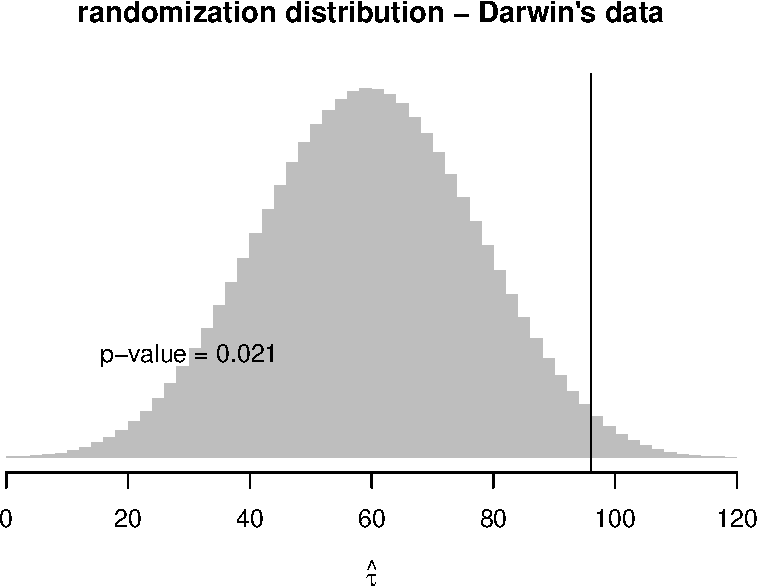
\includegraphics{hw3_files/figure-latex/unnamed-chunk-1-1.pdf}

\begin{Shaded}
\begin{Highlighting}[]
\CommentTok{# Neymanian Inference}
\NormalTok{tau_hat =}\StringTok{ }\KeywordTok{mean}\NormalTok{(ytreat }\OperatorTok{-}\StringTok{ }\NormalTok{ycontrol)}
\NormalTok{V_hat =}\StringTok{ }\KeywordTok{sum}\NormalTok{((ytreat }\OperatorTok{-}\StringTok{ }\NormalTok{ycontrol }\OperatorTok{-}\StringTok{ }\NormalTok{tau_hat)}\OperatorTok{^}\DecValTok{2}\NormalTok{) }\OperatorTok{/}\NormalTok{n.pairs }\OperatorTok{/}\StringTok{ }\NormalTok{(n.pairs}\OperatorTok{-}\DecValTok{1}\NormalTok{)}
\KeywordTok{print}\NormalTok{(}\KeywordTok{paste}\NormalTok{(}\StringTok{"Confidence Interval = ["}\NormalTok{, tau_hat }\OperatorTok{-}\StringTok{ }\FloatTok{1.96}\OperatorTok{*}\KeywordTok{sqrt}\NormalTok{(V_hat), }\StringTok{","}\NormalTok{, tau_hat }\OperatorTok{+}\StringTok{ }\FloatTok{1.96}\OperatorTok{*}\KeywordTok{sqrt}\NormalTok{(V_hat), }\StringTok{"]"}\NormalTok{, }\DataTypeTok{sep =} \StringTok{""}\NormalTok{))}
\end{Highlighting}
\end{Shaded}

\begin{verbatim}
## [1] "Confidence Interval = [1.83204244036545,40.0346242263012]"
\end{verbatim}

\begin{Shaded}
\begin{Highlighting}[]
\NormalTok{## Imbens and Rubin book: matched pair data}
\NormalTok{## television program aimed at improving reading skills for children}
\NormalTok{dataxy =}\StringTok{ }\KeywordTok{c}\NormalTok{(}\FloatTok{12.9}\NormalTok{, }\FloatTok{12.0}\NormalTok{, }\FloatTok{54.6}\NormalTok{, }\FloatTok{60.6}\NormalTok{,}
           \FloatTok{15.1}\NormalTok{, }\FloatTok{12.3}\NormalTok{, }\FloatTok{56.5}\NormalTok{, }\FloatTok{55.5}\NormalTok{,}
           \FloatTok{16.8}\NormalTok{, }\FloatTok{17.2}\NormalTok{, }\FloatTok{75.2}\NormalTok{, }\FloatTok{84.8}\NormalTok{,}
           \FloatTok{15.8}\NormalTok{, }\FloatTok{18.9}\NormalTok{, }\FloatTok{75.6}\NormalTok{, }\FloatTok{101.9}\NormalTok{,}
           \FloatTok{13.9}\NormalTok{, }\FloatTok{15.3}\NormalTok{, }\FloatTok{55.3}\NormalTok{, }\FloatTok{70.6}\NormalTok{,}
           \FloatTok{14.5}\NormalTok{, }\FloatTok{16.6}\NormalTok{, }\FloatTok{59.3}\NormalTok{, }\FloatTok{78.4}\NormalTok{,}
           \FloatTok{17.0}\NormalTok{, }\FloatTok{16.0}\NormalTok{, }\FloatTok{87.0}\NormalTok{, }\FloatTok{84.2}\NormalTok{,}
           \FloatTok{15.8}\NormalTok{, }\FloatTok{20.1}\NormalTok{, }\FloatTok{73.7}\NormalTok{, }\FloatTok{108.6}\NormalTok{)}
           
\NormalTok{dataxy =}\StringTok{ }\KeywordTok{matrix}\NormalTok{(dataxy, }\DecValTok{8}\NormalTok{, }\DecValTok{4}\NormalTok{,  }\DataTypeTok{byrow =} \OtherTok{TRUE}\NormalTok{)           }

\NormalTok{diffx =}\StringTok{ }\NormalTok{dataxy[, }\DecValTok{2}\NormalTok{] }\OperatorTok{-}\StringTok{ }\NormalTok{dataxy[, }\DecValTok{1}\NormalTok{]}
\NormalTok{diffy =}\StringTok{ }\NormalTok{dataxy[, }\DecValTok{4}\NormalTok{] }\OperatorTok{-}\StringTok{ }\NormalTok{dataxy[, }\DecValTok{3}\NormalTok{]}

\NormalTok{dataxy =}\StringTok{ }\KeywordTok{cbind}\NormalTok{(dataxy, diffx, diffy)}

\KeywordTok{rownames}\NormalTok{(dataxy) =}\StringTok{ }\DecValTok{1}\OperatorTok{:}\DecValTok{8}
\KeywordTok{colnames}\NormalTok{(dataxy) =}\StringTok{ }\KeywordTok{c}\NormalTok{(}\StringTok{"x.control"}\NormalTok{, }\StringTok{"x.treatment"}\NormalTok{, }
                     \StringTok{"y.control"}\NormalTok{, }\StringTok{"y.treatment"}\NormalTok{,}
                     \StringTok{"diffx"}\NormalTok{, }\StringTok{"diffy"}\NormalTok{)}
\NormalTok{dataxy}
\end{Highlighting}
\end{Shaded}

\begin{verbatim}
##   x.control x.treatment y.control y.treatment diffx diffy
## 1      12.9        12.0      54.6        60.6  -0.9   6.0
## 2      15.1        12.3      56.5        55.5  -2.8  -1.0
## 3      16.8        17.2      75.2        84.8   0.4   9.6
## 4      15.8        18.9      75.6       101.9   3.1  26.3
## 5      13.9        15.3      55.3        70.6   1.4  15.3
## 6      14.5        16.6      59.3        78.4   2.1  19.1
## 7      17.0        16.0      87.0        84.2  -1.0  -2.8
## 8      15.8        20.1      73.7       108.6   4.3  34.9
\end{verbatim}

\begin{Shaded}
\begin{Highlighting}[]
\NormalTok{ytreat =}\StringTok{ }\NormalTok{dataxy[, }\StringTok{'y.treatment'}\NormalTok{]}
\NormalTok{ycontrol =}\StringTok{ }\NormalTok{dataxy[, }\StringTok{'y.control'}\NormalTok{]}
\NormalTok{difference =}\StringTok{ }\NormalTok{ytreat }\OperatorTok{-}\StringTok{ }\NormalTok{ycontrol}
\NormalTok{n.pairs    =}\StringTok{ }\KeywordTok{length}\NormalTok{(difference)}
\NormalTok{abs.diff   =}\StringTok{ }\KeywordTok{abs}\NormalTok{(difference)}
\NormalTok{t.obs      =}\StringTok{ }\KeywordTok{mean}\NormalTok{(difference)}
\NormalTok{t.ran      =}\StringTok{ }\KeywordTok{sapply}\NormalTok{(}\DecValTok{1}\OperatorTok{:}\DecValTok{2}\OperatorTok{^}\DecValTok{8}\NormalTok{, }
                    \ControlFlowTok{function}\NormalTok{(x)\{ }
                      \KeywordTok{sum}\NormalTok{(}\KeywordTok{MP_enumerate}\NormalTok{(x, }\DecValTok{8}\NormalTok{)}\OperatorTok{*}\NormalTok{abs.diff) }
\NormalTok{                      \})}\OperatorTok{/}\NormalTok{n.pairs}
\NormalTok{w.obs =}\StringTok{ }\KeywordTok{wilcox.test}\NormalTok{(ytreat, ycontrol, }\DataTypeTok{paired =} \OtherTok{TRUE}\NormalTok{)}\OperatorTok{\$}\NormalTok{statistic}
\NormalTok{w.ran      =}\StringTok{ }\KeywordTok{sapply}\NormalTok{(}\DecValTok{1}\OperatorTok{:}\DecValTok{2}\OperatorTok{^}\DecValTok{8}\NormalTok{, }
                    \ControlFlowTok{function}\NormalTok{(x)\{ }
                      \KeywordTok{wilcox.test}\NormalTok{(ytreat}\OperatorTok{*}\NormalTok{(}\OperatorTok{-}\KeywordTok{MP_enumerate}\NormalTok{(x, }\DecValTok{8}\NormalTok{)), ycontrol}\OperatorTok{*}\NormalTok{(}\KeywordTok{MP_enumerate}\NormalTok{(x, }\DecValTok{8}\NormalTok{)), }\DataTypeTok{paired =} \OtherTok{TRUE}\NormalTok{)}\OperatorTok{\$}\NormalTok{statistic}
\NormalTok{                      \}, }\DataTypeTok{simplify =} \OtherTok{TRUE}\NormalTok{)}
\NormalTok{pvalue     =}\StringTok{ }\KeywordTok{mean}\NormalTok{(t.ran}\OperatorTok{>=}\NormalTok{t.obs)}
\NormalTok{pvalue}
\end{Highlighting}
\end{Shaded}

\begin{verbatim}
## [1] 0.015625
\end{verbatim}

\begin{Shaded}
\begin{Highlighting}[]
\NormalTok{pw =}\StringTok{ }\KeywordTok{mean}\NormalTok{(w.ran }\OperatorTok{>=}\StringTok{ }\NormalTok{w.obs)}
\NormalTok{pw}
\end{Highlighting}
\end{Shaded}

\begin{verbatim}
## [1] 0.01953125
\end{verbatim}

\begin{Shaded}
\begin{Highlighting}[]
\KeywordTok{hist}\NormalTok{(t.ran, }\DataTypeTok{breaks =} \DecValTok{50}\NormalTok{, }\DataTypeTok{col =} \StringTok{"grey"}\NormalTok{, }\DataTypeTok{border =} \OtherTok{NA}\NormalTok{,}
     \DataTypeTok{xlab =} \KeywordTok{expression}\NormalTok{(}\KeywordTok{hat}\NormalTok{(tau)), }
     \DataTypeTok{ylab =} \StringTok{""}\NormalTok{, }\DataTypeTok{yaxt =} \StringTok{'n'}\NormalTok{, }
     \DataTypeTok{main =} \StringTok{"randomization distribution - MPstar data"}\NormalTok{)}
\KeywordTok{abline}\NormalTok{(}\DataTypeTok{v =}\NormalTok{ t.obs)}
\KeywordTok{text}\NormalTok{(}\DecValTok{30}\NormalTok{, }\DecValTok{400}\NormalTok{, }
     \KeywordTok{paste}\NormalTok{(}\StringTok{"p-value = "}\NormalTok{, }\KeywordTok{round}\NormalTok{(pvalue, }\DecValTok{3}\NormalTok{), }\DataTypeTok{sep =} \StringTok{""}\NormalTok{))}
\end{Highlighting}
\end{Shaded}

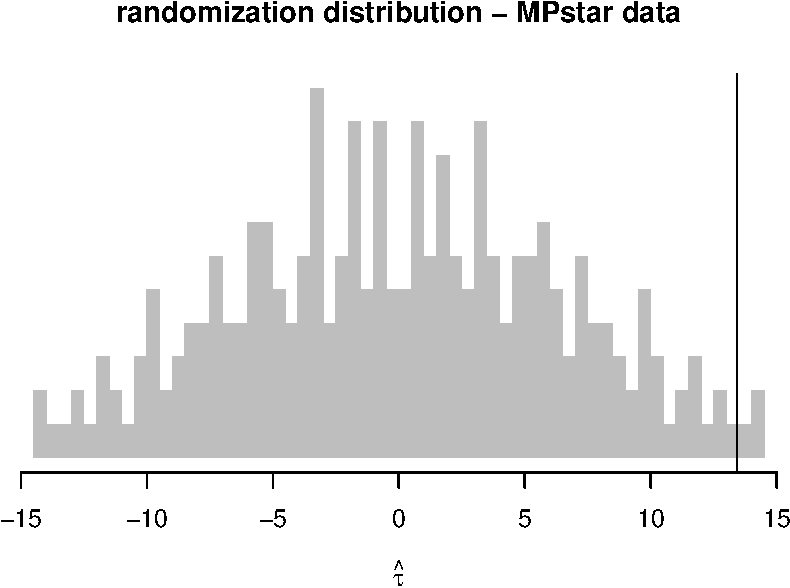
\includegraphics{hw3_files/figure-latex/unnamed-chunk-3-1.pdf}

\begin{Shaded}
\begin{Highlighting}[]
\KeywordTok{hist}\NormalTok{(w.ran, }\DataTypeTok{breaks =} \DecValTok{50}\NormalTok{, }\DataTypeTok{col =} \StringTok{"grey"}\NormalTok{, }\DataTypeTok{border =} \OtherTok{NA}\NormalTok{,}
     \DataTypeTok{xlab =} \KeywordTok{expression}\NormalTok{(}\KeywordTok{hat}\NormalTok{(tau)), }
     \DataTypeTok{ylab =} \StringTok{""}\NormalTok{, }\DataTypeTok{yaxt =} \StringTok{'n'}\NormalTok{, }
     \DataTypeTok{main =} \StringTok{"randomization distribution - MPstar data"}\NormalTok{)}
\KeywordTok{abline}\NormalTok{(}\DataTypeTok{v =}\NormalTok{ w.obs)}
\KeywordTok{text}\NormalTok{(}\DecValTok{30}\NormalTok{, }\DecValTok{400}\NormalTok{, }
     \KeywordTok{paste}\NormalTok{(}\StringTok{"p-value = "}\NormalTok{, }\KeywordTok{round}\NormalTok{(pvalue, }\DecValTok{3}\NormalTok{), }\DataTypeTok{sep =} \StringTok{""}\NormalTok{))}
\end{Highlighting}
\end{Shaded}

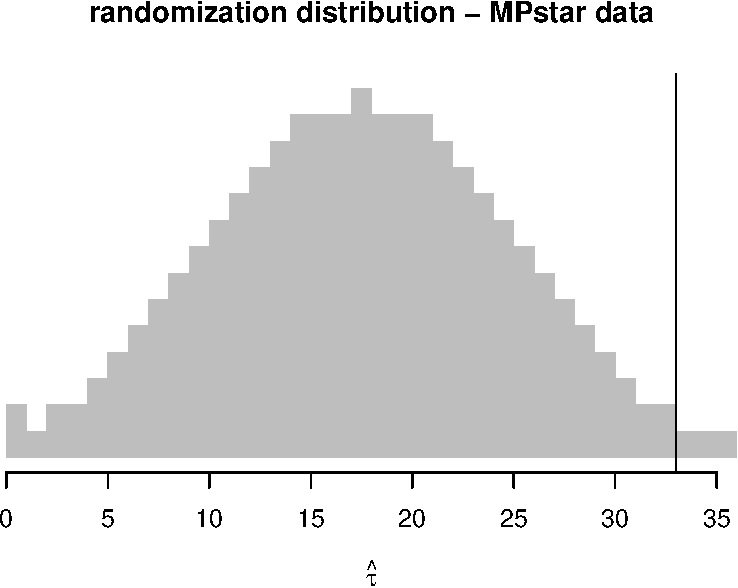
\includegraphics{hw3_files/figure-latex/unnamed-chunk-3-2.pdf}

\begin{Shaded}
\begin{Highlighting}[]
\CommentTok{# Regression Adjustment}
\NormalTok{ycontrol =}\StringTok{ }\KeywordTok{lm}\NormalTok{(y.control}\OperatorTok{~}\NormalTok{x.control, }\DataTypeTok{data =} \KeywordTok{data.frame}\NormalTok{(}\DataTypeTok{y.control =}\NormalTok{ dataxy[,}\StringTok{'y.control'}\NormalTok{], }\DataTypeTok{x.control =}\NormalTok{ dataxy[,}\StringTok{'x.control'}\NormalTok{]))}\OperatorTok{\$}\NormalTok{residuals}
\NormalTok{ytreat =}\StringTok{ }\KeywordTok{lm}\NormalTok{(y.treat}\OperatorTok{~}\NormalTok{x.treat, }\DataTypeTok{data =} \KeywordTok{data.frame}\NormalTok{(}\DataTypeTok{y.treat =}\NormalTok{ dataxy[,}\StringTok{'y.treatment'}\NormalTok{], }\DataTypeTok{x.treat =}\NormalTok{ dataxy[,}\StringTok{'x.treatment'}\NormalTok{]))}\OperatorTok{\$}\NormalTok{residuals}
\NormalTok{difference =}\StringTok{ }\NormalTok{ytreat }\OperatorTok{-}\StringTok{ }\NormalTok{ycontrol}
\NormalTok{n.pairs    =}\StringTok{ }\KeywordTok{length}\NormalTok{(difference)}
\NormalTok{abs.diff   =}\StringTok{ }\KeywordTok{abs}\NormalTok{(difference)}
\NormalTok{t.obs      =}\StringTok{ }\KeywordTok{mean}\NormalTok{(difference)}
\NormalTok{t.ran      =}\StringTok{ }\KeywordTok{sapply}\NormalTok{(}\DecValTok{1}\OperatorTok{:}\DecValTok{2}\OperatorTok{^}\DecValTok{8}\NormalTok{, }
                    \ControlFlowTok{function}\NormalTok{(x)\{ }
                      \KeywordTok{sum}\NormalTok{(}\KeywordTok{MP_enumerate}\NormalTok{(x, }\DecValTok{8}\NormalTok{)}\OperatorTok{*}\NormalTok{abs.diff) }
\NormalTok{                      \})}\OperatorTok{/}\NormalTok{n.pairs}
\NormalTok{w.obs =}\StringTok{ }\KeywordTok{wilcox.test}\NormalTok{(ytreat, ycontrol, }\DataTypeTok{paired =} \OtherTok{TRUE}\NormalTok{)}\OperatorTok{\$}\NormalTok{statistic}
\NormalTok{w.ran      =}\StringTok{ }\KeywordTok{sapply}\NormalTok{(}\DecValTok{1}\OperatorTok{:}\DecValTok{2}\OperatorTok{^}\DecValTok{8}\NormalTok{, }
                    \ControlFlowTok{function}\NormalTok{(x)\{ }
                      \KeywordTok{wilcox.test}\NormalTok{(ytreat}\OperatorTok{*}\NormalTok{(}\OperatorTok{-}\KeywordTok{MP_enumerate}\NormalTok{(x, }\DecValTok{8}\NormalTok{)), ycontrol}\OperatorTok{*}\NormalTok{(}\KeywordTok{MP_enumerate}\NormalTok{(x, }\DecValTok{8}\NormalTok{)), }\DataTypeTok{paired =} \OtherTok{TRUE}\NormalTok{)}\OperatorTok{\$}\NormalTok{statistic}
\NormalTok{                      \}, }\DataTypeTok{simplify =} \OtherTok{TRUE}\NormalTok{)}
\NormalTok{pvalue     =}\StringTok{ }\KeywordTok{mean}\NormalTok{(t.ran}\OperatorTok{>=}\NormalTok{t.obs)}
\NormalTok{pvalue}
\end{Highlighting}
\end{Shaded}

\begin{verbatim}
## [1] 0.5
\end{verbatim}

\begin{Shaded}
\begin{Highlighting}[]
\NormalTok{pw =}\StringTok{ }\KeywordTok{mean}\NormalTok{(w.ran }\OperatorTok{>=}\StringTok{ }\NormalTok{w.obs)}
\NormalTok{pw}
\end{Highlighting}
\end{Shaded}

\begin{verbatim}
## [1] 0.6796875
\end{verbatim}

\begin{Shaded}
\begin{Highlighting}[]
\KeywordTok{hist}\NormalTok{(t.ran, }\DataTypeTok{breaks =} \DecValTok{50}\NormalTok{, }\DataTypeTok{col =} \StringTok{"grey"}\NormalTok{, }\DataTypeTok{border =} \OtherTok{NA}\NormalTok{,}
     \DataTypeTok{xlab =} \KeywordTok{expression}\NormalTok{(}\KeywordTok{hat}\NormalTok{(tau)), }
     \DataTypeTok{ylab =} \StringTok{""}\NormalTok{, }\DataTypeTok{yaxt =} \StringTok{'n'}\NormalTok{, }
     \DataTypeTok{main =} \StringTok{"randomization distribution - MPstar data"}\NormalTok{)}
\KeywordTok{abline}\NormalTok{(}\DataTypeTok{v =}\NormalTok{ t.obs)}
\KeywordTok{text}\NormalTok{(}\DecValTok{30}\NormalTok{, }\DecValTok{400}\NormalTok{, }
     \KeywordTok{paste}\NormalTok{(}\StringTok{"p-value = "}\NormalTok{, }\KeywordTok{round}\NormalTok{(pvalue, }\DecValTok{3}\NormalTok{), }\DataTypeTok{sep =} \StringTok{""}\NormalTok{))}
\end{Highlighting}
\end{Shaded}

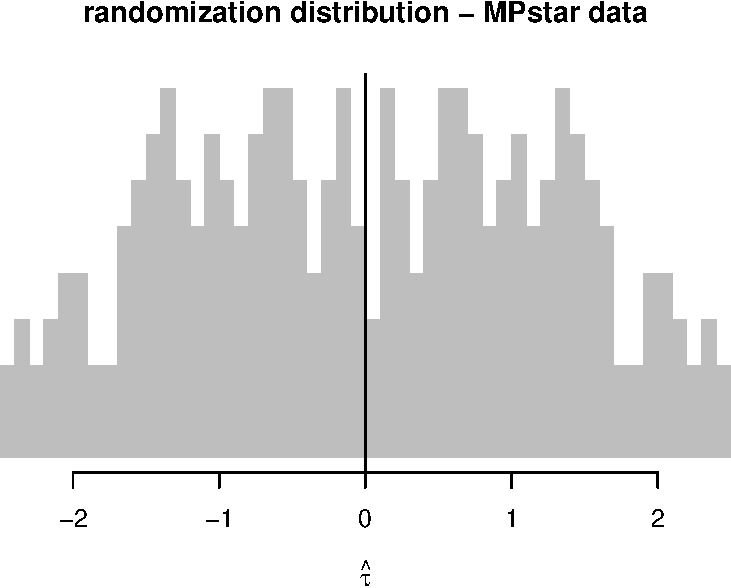
\includegraphics{hw3_files/figure-latex/unnamed-chunk-4-1.pdf}

\begin{Shaded}
\begin{Highlighting}[]
\KeywordTok{hist}\NormalTok{(w.ran, }\DataTypeTok{breaks =} \DecValTok{50}\NormalTok{, }\DataTypeTok{col =} \StringTok{"grey"}\NormalTok{, }\DataTypeTok{border =} \OtherTok{NA}\NormalTok{,}
     \DataTypeTok{xlab =} \KeywordTok{expression}\NormalTok{(}\KeywordTok{hat}\NormalTok{(tau)), }
     \DataTypeTok{ylab =} \StringTok{""}\NormalTok{, }\DataTypeTok{yaxt =} \StringTok{'n'}\NormalTok{, }
     \DataTypeTok{main =} \StringTok{"randomization distribution - MPstar data"}\NormalTok{)}
\KeywordTok{abline}\NormalTok{(}\DataTypeTok{v =}\NormalTok{ w.obs)}
\KeywordTok{text}\NormalTok{(}\DecValTok{30}\NormalTok{, }\DecValTok{400}\NormalTok{, }
     \KeywordTok{paste}\NormalTok{(}\StringTok{"p-value = "}\NormalTok{, }\KeywordTok{round}\NormalTok{(pvalue, }\DecValTok{3}\NormalTok{), }\DataTypeTok{sep =} \StringTok{""}\NormalTok{))}
\end{Highlighting}
\end{Shaded}

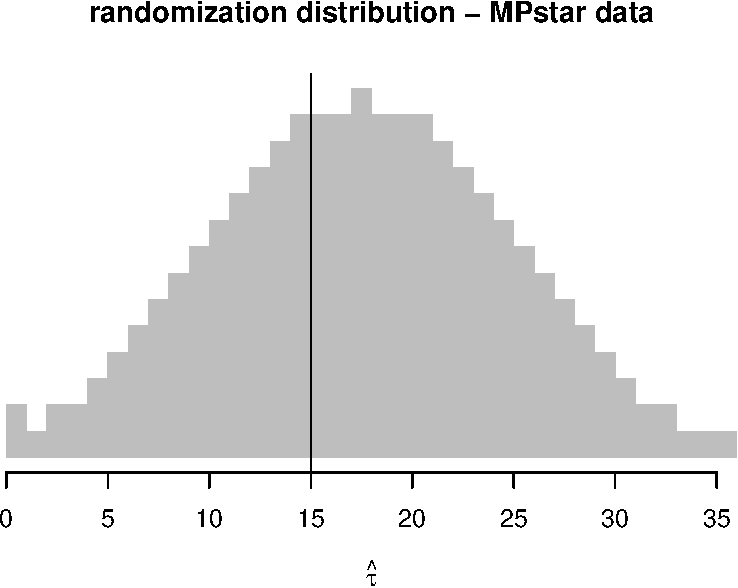
\includegraphics{hw3_files/figure-latex/unnamed-chunk-4-2.pdf}

\begin{Shaded}
\begin{Highlighting}[]
\CommentTok{# Data Input}
\NormalTok{dataxy =}\StringTok{ }\KeywordTok{c}\NormalTok{(.}\DecValTok{046}\NormalTok{, }\DecValTok{0}\NormalTok{, .}\DecValTok{091}\NormalTok{, .}\DecValTok{185}\NormalTok{, .}\DecValTok{036}\NormalTok{, .}\DecValTok{051}\NormalTok{, }\DecValTok{0}\NormalTok{, .}\DecValTok{047}\NormalTok{,}
\NormalTok{           .}\DecValTok{054}\NormalTok{, .}\DecValTok{094}\NormalTok{, .}\DecValTok{184}\NormalTok{, .}\DecValTok{034}\NormalTok{, .}\DecValTok{05}\NormalTok{, .}\DecValTok{108}\NormalTok{, .}\DecValTok{11}\NormalTok{, .}\DecValTok{095}\NormalTok{,}
\NormalTok{           .}\DecValTok{114}\NormalTok{, }\DecValTok{0}\NormalTok{, .}\DecValTok{056}\NormalTok{, .}\DecValTok{075}\NormalTok{, .}\DecValTok{098}\NormalTok{, .}\DecValTok{054}\NormalTok{, .}\DecValTok{030}\NormalTok{, .}\DecValTok{068}\NormalTok{,}
\NormalTok{           .}\DecValTok{148}\NormalTok{, .}\DecValTok{162}\NormalTok{, .}\DecValTok{082}\NormalTok{, .}\DecValTok{075}\NormalTok{, .}\DecValTok{134}\NormalTok{, .}\DecValTok{39}\NormalTok{, .}\DecValTok{339}\NormalTok{, .}\DecValTok{458}\NormalTok{,}
\NormalTok{           .}\DecValTok{152}\NormalTok{, .}\DecValTok{105}\NormalTok{, .}\DecValTok{083}\NormalTok{, .}\DecValTok{129}\NormalTok{, .}\DecValTok{145}\NormalTok{, .}\DecValTok{077}\NormalTok{, .}\DecValTok{579}\NormalTok{, .}\DecValTok{167}\NormalTok{, }
\NormalTok{           .}\DecValTok{188}\NormalTok{, .}\DecValTok{214}\NormalTok{, .}\DecValTok{375}\NormalTok{, .}\DecValTok{545}\NormalTok{, .}\DecValTok{179}\NormalTok{, .}\DecValTok{165}\NormalTok{, .}\DecValTok{483}\NormalTok{, .}\DecValTok{444}\NormalTok{,}
\NormalTok{           .}\DecValTok{193}\NormalTok{, .}\DecValTok{771}\NormalTok{, .}\DecValTok{328}\NormalTok{, .}\DecValTok{583}\NormalTok{, .}\DecValTok{189}\NormalTok{, .}\DecValTok{186}\NormalTok{, .}\DecValTok{168}\NormalTok{, .}\DecValTok{368}\NormalTok{,}
\NormalTok{           .}\DecValTok{197}\NormalTok{, .}\DecValTok{350}\NormalTok{, .}\DecValTok{0}\NormalTok{, .}\DecValTok{383}\NormalTok{, .}\DecValTok{2}\NormalTok{, .}\DecValTok{071}\NormalTok{, .}\DecValTok{667}\NormalTok{, .}\DecValTok{429}\NormalTok{,}
\NormalTok{           .}\DecValTok{213}\NormalTok{, .}\DecValTok{176}\NormalTok{, .}\DecValTok{164}\NormalTok{, .}\DecValTok{172}\NormalTok{, .}\DecValTok{209}\NormalTok{, .}\DecValTok{165}\NormalTok{, .}\DecValTok{092}\NormalTok{, .}\DecValTok{151}\NormalTok{,}
\NormalTok{           .}\DecValTok{211}\NormalTok{, .}\DecValTok{667}\NormalTok{, .}\DecValTok{25}\NormalTok{, .}\DecValTok{617}\NormalTok{, .}\DecValTok{219}\NormalTok{, .}\DecValTok{25}\NormalTok{, .}\DecValTok{5}\NormalTok{, .}\DecValTok{35}\NormalTok{,}
\NormalTok{           .}\DecValTok{219}\NormalTok{, .}\DecValTok{153}\NormalTok{, .}\DecValTok{185}\NormalTok{, .}\DecValTok{219}\NormalTok{, .}\DecValTok{224}\NormalTok{, .}\DecValTok{363}\NormalTok{, .}\DecValTok{372}\NormalTok{, .}\DecValTok{342}\NormalTok{,}
\NormalTok{           .}\DecValTok{255}\NormalTok{, .}\DecValTok{226}\NormalTok{, .}\DecValTok{213}\NormalTok{, .}\DecValTok{327}\NormalTok{, .}\DecValTok{257}\NormalTok{, .}\DecValTok{098}\NormalTok{, .}\DecValTok{107}\NormalTok{, .}\DecValTok{095}\NormalTok{,}
\NormalTok{           .}\DecValTok{261}\NormalTok{, .}\DecValTok{071}\NormalTok{, .}\DecValTok{0}\NormalTok{, .}\DecValTok{435}\NormalTok{, .}\DecValTok{263}\NormalTok{, .}\DecValTok{441}\NormalTok{, .}\DecValTok{448}\NormalTok{, .}\DecValTok{435}\NormalTok{,}
\NormalTok{           .}\DecValTok{286}\NormalTok{, .}\DecValTok{161}\NormalTok{, .}\DecValTok{126}\NormalTok{, .}\DecValTok{181}\NormalTok{, .}\DecValTok{285}\NormalTok{, .}\DecValTok{389}\NormalTok{, .}\DecValTok{353}\NormalTok{, .}\DecValTok{309}\NormalTok{)}
\NormalTok{data <-}\StringTok{ }\KeywordTok{data.frame}\NormalTok{(}\KeywordTok{matrix}\NormalTok{(dataxy, }\DataTypeTok{ncol =} \DecValTok{4}\NormalTok{))}
\NormalTok{data <-}\StringTok{ }\NormalTok{data }\OperatorTok{\%>\%}
\StringTok{  }\KeywordTok{rename}\NormalTok{(}\DataTypeTok{Y1 =}\NormalTok{ X3, }\DataTypeTok{Y2 =}\NormalTok{ X4) }\OperatorTok{\%>\%}
\StringTok{  }\KeywordTok{mutate}\NormalTok{(}\DataTypeTok{Y =}\NormalTok{ Y1 }\OperatorTok{+}\StringTok{ }\NormalTok{Y2)}
\end{Highlighting}
\end{Shaded}

\begin{Shaded}
\begin{Highlighting}[]
\CommentTok{# FRT with raw data}
\NormalTok{data <-}\StringTok{ }\NormalTok{data }\OperatorTok{\%>\%}
\StringTok{  }\KeywordTok{mutate}\NormalTok{(}\DataTypeTok{index =} \DecValTok{1}\OperatorTok{:}\DecValTok{28}\NormalTok{) }\OperatorTok{\%>\%}
\StringTok{  }\KeywordTok{mutate}\NormalTok{(}\DataTypeTok{pair =}\NormalTok{ (index}\OperatorTok{+}\DecValTok{1}\NormalTok{) }\OperatorTok{\%/\%}\StringTok{ }\DecValTok{2}\NormalTok{) }\OperatorTok{\%>\%}
\StringTok{  }\KeywordTok{mutate}\NormalTok{(}\DataTypeTok{z =}\NormalTok{ (index}\OperatorTok{+}\DecValTok{1}\NormalTok{) }\OperatorTok{\%\%}\StringTok{ }\DecValTok{2}\NormalTok{) }\OperatorTok{\%>\%}
\StringTok{  }\KeywordTok{select}\NormalTok{(}\OperatorTok{-}\NormalTok{index, }\OperatorTok{-}\NormalTok{Y1, }\OperatorTok{-}\NormalTok{Y2)}
\NormalTok{stat_Pair <-}\StringTok{ }\ControlFlowTok{function}\NormalTok{(pair, treatment, y)\{}
  \CommentTok{# Assume in our case that the stratum in arranged and indexed.}
  \CommentTok{# If not, then re-code it to an index.}
\NormalTok{  number =}\StringTok{ }\KeywordTok{length}\NormalTok{(}\KeywordTok{unique}\NormalTok{(pair))}
\NormalTok{  tau =}\StringTok{ }\DecValTok{0}
\NormalTok{  temptau =}\StringTok{ }\KeywordTok{rep}\NormalTok{(}\DecValTok{0}\NormalTok{, number)}
\NormalTok{  wil =}\StringTok{ }\DecValTok{0}
\NormalTok{  sign =}\StringTok{ }\DecValTok{0}
  \CommentTok{# Calculate the three statistics as defined}
  \ControlFlowTok{for}\NormalTok{ (i }\ControlFlowTok{in} \DecValTok{1}\OperatorTok{:}\NormalTok{number)\{}
\NormalTok{    tempy =}\StringTok{ }\NormalTok{y[pair }\OperatorTok{==}\StringTok{ }\NormalTok{i]}
\NormalTok{    tempt =}\StringTok{ }\NormalTok{treatment[pair }\OperatorTok{==}\StringTok{ }\NormalTok{i]}
\NormalTok{    tau =}\StringTok{ }\NormalTok{tau }\OperatorTok{+}\StringTok{ }\NormalTok{(tempy[tempt }\OperatorTok{==}\StringTok{ }\DecValTok{1}\NormalTok{] }\OperatorTok{-}\StringTok{ }\NormalTok{tempy[tempt }\OperatorTok{==}\StringTok{ }\DecValTok{0}\NormalTok{])}\OperatorTok{/}\NormalTok{number}
\NormalTok{    temptau[i] =}\StringTok{ }\NormalTok{tempy[tempt }\OperatorTok{==}\StringTok{ }\DecValTok{1}\NormalTok{] }\OperatorTok{-}\StringTok{ }\NormalTok{tempy[tempt }\OperatorTok{==}\StringTok{ }\DecValTok{0}\NormalTok{]}
\NormalTok{    sign =}\StringTok{ }\NormalTok{sign }\OperatorTok{+}\StringTok{ }\KeywordTok{ifelse}\NormalTok{(tempy[tempt }\OperatorTok{==}\StringTok{ }\DecValTok{1}\NormalTok{] }\OperatorTok{>}\StringTok{ }\NormalTok{tempy[tempt }\OperatorTok{==}\StringTok{ }\DecValTok{0}\NormalTok{], }\DecValTok{1}\NormalTok{, }\DecValTok{0}\NormalTok{)}
\NormalTok{  \}}
\NormalTok{  Wrank =}\StringTok{ }\KeywordTok{rank}\NormalTok{(temptau)}
  \ControlFlowTok{for}\NormalTok{ (i }\ControlFlowTok{in} \DecValTok{1}\OperatorTok{:}\NormalTok{number)\{}
\NormalTok{    tempy =}\StringTok{ }\NormalTok{y[pair }\OperatorTok{==}\StringTok{ }\NormalTok{i]}
\NormalTok{    tempt =}\StringTok{ }\NormalTok{treatment[pair }\OperatorTok{==}\StringTok{ }\NormalTok{i]}
\NormalTok{    wil =}\StringTok{ }\NormalTok{wil }\OperatorTok{+}\StringTok{ }\KeywordTok{ifelse}\NormalTok{(tempy[tempt }\OperatorTok{==}\StringTok{ }\DecValTok{1}\NormalTok{] }\OperatorTok{>}\StringTok{ }\NormalTok{tempy[tempt }\OperatorTok{==}\StringTok{ }\DecValTok{0}\NormalTok{], }\DecValTok{1}\NormalTok{, }\DecValTok{0}\NormalTok{)}\OperatorTok{*}\NormalTok{Wrank[i]}
\NormalTok{  \}}
  \KeywordTok{return}\NormalTok{(}\KeywordTok{c}\NormalTok{(}\DataTypeTok{taus =}\NormalTok{ tau, }\DataTypeTok{wilcoxon =}\NormalTok{ wil, }\DataTypeTok{alignedRank =}\NormalTok{ sign))}
\NormalTok{\}}
\NormalTok{obsValue <-}\StringTok{ }\KeywordTok{stat_Pair}\NormalTok{(data}\OperatorTok{\$}\NormalTok{pair, data}\OperatorTok{\$}\NormalTok{z, data}\OperatorTok{\$}\NormalTok{Y)}
\end{Highlighting}
\end{Shaded}

\begin{Shaded}
\begin{Highlighting}[]
\NormalTok{ext =}\StringTok{ }\KeywordTok{rep}\NormalTok{(}\DecValTok{0}\NormalTok{,}\DecValTok{3}\NormalTok{)}
\ControlFlowTok{for}\NormalTok{ (i }\ControlFlowTok{in} \DecValTok{1}\OperatorTok{:}\NormalTok{MC)\{}
\NormalTok{  rvalue =}\StringTok{ }\KeywordTok{stat_Pair}\NormalTok{(data}\OperatorTok{\$}\NormalTok{pair, }\KeywordTok{permute}\NormalTok{(data}\OperatorTok{\$}\NormalTok{pair, data}\OperatorTok{\$}\NormalTok{z), data}\OperatorTok{\$}\NormalTok{Y)}
  \ControlFlowTok{for}\NormalTok{ (j }\ControlFlowTok{in} \DecValTok{1}\OperatorTok{:}\DecValTok{3}\NormalTok{)\{}
    \ControlFlowTok{if}\NormalTok{ (}\KeywordTok{abs}\NormalTok{(obsValue[j]) }\OperatorTok{>}\StringTok{ }\KeywordTok{abs}\NormalTok{(rvalue[j]))\{}
\NormalTok{      ext[j] =}\StringTok{ }\NormalTok{ext[j]}\OperatorTok{+}\DecValTok{1}
\NormalTok{    \}}
\NormalTok{  \}}
\NormalTok{\}}
\NormalTok{ext}\OperatorTok{/}\NormalTok{MC}
\end{Highlighting}
\end{Shaded}

\begin{verbatim}
## [1] 0.742 0.226 0.226
\end{verbatim}

\begin{Shaded}
\begin{Highlighting}[]
\CommentTok{# FRT with covariate-adjusted data}
\NormalTok{dataxy =}\StringTok{ }\KeywordTok{c}\NormalTok{(.}\DecValTok{046}\NormalTok{, }\DecValTok{0}\NormalTok{, .}\DecValTok{091}\NormalTok{, .}\DecValTok{185}\NormalTok{, .}\DecValTok{036}\NormalTok{, .}\DecValTok{051}\NormalTok{, }\DecValTok{0}\NormalTok{, .}\DecValTok{047}\NormalTok{,}
\NormalTok{           .}\DecValTok{054}\NormalTok{, .}\DecValTok{094}\NormalTok{, .}\DecValTok{184}\NormalTok{, .}\DecValTok{034}\NormalTok{, .}\DecValTok{05}\NormalTok{, .}\DecValTok{108}\NormalTok{, .}\DecValTok{11}\NormalTok{, .}\DecValTok{095}\NormalTok{,}
\NormalTok{           .}\DecValTok{114}\NormalTok{, }\DecValTok{0}\NormalTok{, .}\DecValTok{056}\NormalTok{, .}\DecValTok{075}\NormalTok{, .}\DecValTok{098}\NormalTok{, .}\DecValTok{054}\NormalTok{, .}\DecValTok{030}\NormalTok{, .}\DecValTok{068}\NormalTok{,}
\NormalTok{           .}\DecValTok{148}\NormalTok{, .}\DecValTok{162}\NormalTok{, .}\DecValTok{082}\NormalTok{, .}\DecValTok{075}\NormalTok{, .}\DecValTok{134}\NormalTok{, .}\DecValTok{39}\NormalTok{, .}\DecValTok{339}\NormalTok{, .}\DecValTok{458}\NormalTok{,}
\NormalTok{           .}\DecValTok{152}\NormalTok{, .}\DecValTok{105}\NormalTok{, .}\DecValTok{083}\NormalTok{, .}\DecValTok{129}\NormalTok{, .}\DecValTok{145}\NormalTok{, .}\DecValTok{077}\NormalTok{, .}\DecValTok{579}\NormalTok{, .}\DecValTok{167}\NormalTok{, }
\NormalTok{           .}\DecValTok{188}\NormalTok{, .}\DecValTok{214}\NormalTok{, .}\DecValTok{375}\NormalTok{, .}\DecValTok{545}\NormalTok{, .}\DecValTok{179}\NormalTok{, .}\DecValTok{165}\NormalTok{, .}\DecValTok{483}\NormalTok{, .}\DecValTok{444}\NormalTok{,}
\NormalTok{           .}\DecValTok{193}\NormalTok{, .}\DecValTok{771}\NormalTok{, .}\DecValTok{328}\NormalTok{, .}\DecValTok{583}\NormalTok{, .}\DecValTok{189}\NormalTok{, .}\DecValTok{186}\NormalTok{, .}\DecValTok{168}\NormalTok{, .}\DecValTok{368}\NormalTok{,}
\NormalTok{           .}\DecValTok{197}\NormalTok{, .}\DecValTok{350}\NormalTok{, .}\DecValTok{0}\NormalTok{, .}\DecValTok{383}\NormalTok{, .}\DecValTok{2}\NormalTok{, .}\DecValTok{071}\NormalTok{, .}\DecValTok{667}\NormalTok{, .}\DecValTok{429}\NormalTok{,}
\NormalTok{           .}\DecValTok{213}\NormalTok{, .}\DecValTok{176}\NormalTok{, .}\DecValTok{164}\NormalTok{, .}\DecValTok{172}\NormalTok{, .}\DecValTok{209}\NormalTok{, .}\DecValTok{165}\NormalTok{, .}\DecValTok{092}\NormalTok{, .}\DecValTok{151}\NormalTok{,}
\NormalTok{           .}\DecValTok{211}\NormalTok{, .}\DecValTok{667}\NormalTok{, .}\DecValTok{25}\NormalTok{, .}\DecValTok{617}\NormalTok{, .}\DecValTok{219}\NormalTok{, .}\DecValTok{25}\NormalTok{, .}\DecValTok{5}\NormalTok{, .}\DecValTok{35}\NormalTok{,}
\NormalTok{           .}\DecValTok{219}\NormalTok{, .}\DecValTok{153}\NormalTok{, .}\DecValTok{185}\NormalTok{, .}\DecValTok{219}\NormalTok{, .}\DecValTok{224}\NormalTok{, .}\DecValTok{363}\NormalTok{, .}\DecValTok{372}\NormalTok{, .}\DecValTok{342}\NormalTok{,}
\NormalTok{           .}\DecValTok{255}\NormalTok{, .}\DecValTok{226}\NormalTok{, .}\DecValTok{213}\NormalTok{, .}\DecValTok{327}\NormalTok{, .}\DecValTok{257}\NormalTok{, .}\DecValTok{098}\NormalTok{, .}\DecValTok{107}\NormalTok{, .}\DecValTok{095}\NormalTok{,}
\NormalTok{           .}\DecValTok{261}\NormalTok{, .}\DecValTok{071}\NormalTok{, .}\DecValTok{0}\NormalTok{, .}\DecValTok{435}\NormalTok{, .}\DecValTok{263}\NormalTok{, .}\DecValTok{441}\NormalTok{, .}\DecValTok{448}\NormalTok{, .}\DecValTok{435}\NormalTok{,}
\NormalTok{           .}\DecValTok{286}\NormalTok{, .}\DecValTok{161}\NormalTok{, .}\DecValTok{126}\NormalTok{, .}\DecValTok{181}\NormalTok{, .}\DecValTok{285}\NormalTok{, .}\DecValTok{389}\NormalTok{, .}\DecValTok{353}\NormalTok{, .}\DecValTok{309}\NormalTok{)}
\NormalTok{data <-}\StringTok{ }\KeywordTok{data.frame}\NormalTok{(}\KeywordTok{matrix}\NormalTok{(dataxy, }\DataTypeTok{ncol =} \DecValTok{4}\NormalTok{))}
\NormalTok{data <-}\StringTok{ }\NormalTok{data }\OperatorTok{\%>\%}
\StringTok{  }\KeywordTok{rename}\NormalTok{(}\DataTypeTok{Y1 =}\NormalTok{ X3, }\DataTypeTok{Y2 =}\NormalTok{ X4) }\OperatorTok{\%>\%}
\StringTok{  }\KeywordTok{mutate}\NormalTok{(}\DataTypeTok{Y =} \KeywordTok{lm}\NormalTok{((Y1}\OperatorTok{+}\NormalTok{Y2)}\OperatorTok{~}\NormalTok{X1}\OperatorTok{+}\NormalTok{X2)}\OperatorTok{\$}\NormalTok{residuals)}
\end{Highlighting}
\end{Shaded}

\begin{Shaded}
\begin{Highlighting}[]
\NormalTok{data <-}\StringTok{ }\NormalTok{data }\OperatorTok{\%>\%}
\StringTok{  }\KeywordTok{mutate}\NormalTok{(}\DataTypeTok{index =} \DecValTok{1}\OperatorTok{:}\DecValTok{28}\NormalTok{) }\OperatorTok{\%>\%}
\StringTok{  }\KeywordTok{mutate}\NormalTok{(}\DataTypeTok{pair =}\NormalTok{ (index}\OperatorTok{+}\DecValTok{1}\NormalTok{) }\OperatorTok{\%/\%}\StringTok{ }\DecValTok{2}\NormalTok{) }\OperatorTok{\%>\%}
\StringTok{  }\KeywordTok{mutate}\NormalTok{(}\DataTypeTok{z =}\NormalTok{ (index}\OperatorTok{+}\DecValTok{1}\NormalTok{) }\OperatorTok{\%\%}\StringTok{ }\DecValTok{2}\NormalTok{) }\OperatorTok{\%>\%}
\StringTok{  }\KeywordTok{select}\NormalTok{(}\OperatorTok{-}\NormalTok{index, }\OperatorTok{-}\NormalTok{Y1, }\OperatorTok{-}\NormalTok{Y2)}
\NormalTok{stat_Pair <-}\StringTok{ }\ControlFlowTok{function}\NormalTok{(pair, treatment, y)\{}
  \CommentTok{# Assume in our case that the stratum in arranged and indexed.}
  \CommentTok{# If not, then re-code it to an index.}
\NormalTok{  number =}\StringTok{ }\KeywordTok{length}\NormalTok{(}\KeywordTok{unique}\NormalTok{(pair))}
\NormalTok{  tau =}\StringTok{ }\DecValTok{0}
\NormalTok{  temptau =}\StringTok{ }\KeywordTok{rep}\NormalTok{(}\DecValTok{0}\NormalTok{, number)}
\NormalTok{  wil =}\StringTok{ }\DecValTok{0}
\NormalTok{  sign =}\StringTok{ }\DecValTok{0}
  \CommentTok{# Calculate the three statistics as defined}
  \ControlFlowTok{for}\NormalTok{ (i }\ControlFlowTok{in} \DecValTok{1}\OperatorTok{:}\NormalTok{number)\{}
\NormalTok{    tempy =}\StringTok{ }\NormalTok{y[pair }\OperatorTok{==}\StringTok{ }\NormalTok{i]}
\NormalTok{    tempt =}\StringTok{ }\NormalTok{treatment[pair }\OperatorTok{==}\StringTok{ }\NormalTok{i]}
\NormalTok{    tau =}\StringTok{ }\NormalTok{tau }\OperatorTok{+}\StringTok{ }\NormalTok{(tempy[tempt }\OperatorTok{==}\StringTok{ }\DecValTok{1}\NormalTok{] }\OperatorTok{-}\StringTok{ }\NormalTok{tempy[tempt }\OperatorTok{==}\StringTok{ }\DecValTok{0}\NormalTok{])}\OperatorTok{/}\NormalTok{number}
\NormalTok{    temptau[i] =}\StringTok{ }\NormalTok{tempy[tempt }\OperatorTok{==}\StringTok{ }\DecValTok{1}\NormalTok{] }\OperatorTok{-}\StringTok{ }\NormalTok{tempy[tempt }\OperatorTok{==}\StringTok{ }\DecValTok{0}\NormalTok{]}
\NormalTok{    sign =}\StringTok{ }\NormalTok{sign }\OperatorTok{+}\StringTok{ }\KeywordTok{ifelse}\NormalTok{(tempy[tempt }\OperatorTok{==}\StringTok{ }\DecValTok{1}\NormalTok{] }\OperatorTok{>}\StringTok{ }\NormalTok{tempy[tempt }\OperatorTok{==}\StringTok{ }\DecValTok{0}\NormalTok{], }\DecValTok{1}\NormalTok{, }\DecValTok{0}\NormalTok{)}
\NormalTok{  \}}
\NormalTok{  Wrank =}\StringTok{ }\KeywordTok{rank}\NormalTok{(temptau)}
  \ControlFlowTok{for}\NormalTok{ (i }\ControlFlowTok{in} \DecValTok{1}\OperatorTok{:}\NormalTok{number)\{}
\NormalTok{    tempy =}\StringTok{ }\NormalTok{y[pair }\OperatorTok{==}\StringTok{ }\NormalTok{i]}
\NormalTok{    tempt =}\StringTok{ }\NormalTok{treatment[pair }\OperatorTok{==}\StringTok{ }\NormalTok{i]}
\NormalTok{    wil =}\StringTok{ }\NormalTok{wil }\OperatorTok{+}\StringTok{ }\KeywordTok{ifelse}\NormalTok{(tempy[tempt }\OperatorTok{==}\StringTok{ }\DecValTok{1}\NormalTok{] }\OperatorTok{>}\StringTok{ }\NormalTok{tempy[tempt }\OperatorTok{==}\StringTok{ }\DecValTok{0}\NormalTok{], }\DecValTok{1}\NormalTok{, }\DecValTok{0}\NormalTok{)}\OperatorTok{*}\NormalTok{Wrank[i]}
\NormalTok{  \}}
  \KeywordTok{return}\NormalTok{(}\KeywordTok{c}\NormalTok{(}\DataTypeTok{taus =}\NormalTok{ tau, }\DataTypeTok{wilcoxon =}\NormalTok{ wil, }\DataTypeTok{alignedRank =}\NormalTok{ sign))}
\NormalTok{\}}
\NormalTok{obsValue <-}\StringTok{ }\KeywordTok{stat_Pair}\NormalTok{(data}\OperatorTok{\$}\NormalTok{pair, data}\OperatorTok{\$}\NormalTok{z, data}\OperatorTok{\$}\NormalTok{Y)}
\end{Highlighting}
\end{Shaded}

\begin{Shaded}
\begin{Highlighting}[]
\NormalTok{ext =}\StringTok{ }\KeywordTok{rep}\NormalTok{(}\DecValTok{0}\NormalTok{,}\DecValTok{3}\NormalTok{)}
\ControlFlowTok{for}\NormalTok{ (i }\ControlFlowTok{in} \DecValTok{1}\OperatorTok{:}\NormalTok{MC)\{}
\NormalTok{  rvalue =}\StringTok{ }\KeywordTok{stat_Pair}\NormalTok{(data}\OperatorTok{\$}\NormalTok{pair, }\KeywordTok{permute}\NormalTok{(data}\OperatorTok{\$}\NormalTok{pair, data}\OperatorTok{\$}\NormalTok{z), data}\OperatorTok{\$}\NormalTok{Y)}
  \ControlFlowTok{for}\NormalTok{ (j }\ControlFlowTok{in} \DecValTok{1}\OperatorTok{:}\DecValTok{3}\NormalTok{)\{}
    \ControlFlowTok{if}\NormalTok{ (}\KeywordTok{abs}\NormalTok{(obsValue[j]) }\OperatorTok{>}\StringTok{ }\KeywordTok{abs}\NormalTok{(rvalue[j]))\{}
\NormalTok{      ext[j] =}\StringTok{ }\NormalTok{ext[j]}\OperatorTok{+}\DecValTok{1}
\NormalTok{    \}}
\NormalTok{  \}}
\NormalTok{\}}
\end{Highlighting}
\end{Shaded}

\begin{Shaded}
\begin{Highlighting}[]
\CommentTok{# Neyman Inference with raw data}
\NormalTok{number =}\StringTok{ }\DecValTok{14}
\NormalTok{temptau =}\StringTok{ }\KeywordTok{rep}\NormalTok{(}\DecValTok{0}\NormalTok{, number)}
\ControlFlowTok{for}\NormalTok{ (i }\ControlFlowTok{in} \DecValTok{1}\OperatorTok{:}\NormalTok{number)\{}
\NormalTok{  tempy =}\StringTok{ }\NormalTok{data}\OperatorTok{\$}\NormalTok{Y[data}\OperatorTok{\$}\NormalTok{pair }\OperatorTok{==}\StringTok{ }\NormalTok{i]}
\NormalTok{  tempt =}\StringTok{ }\NormalTok{data}\OperatorTok{\$}\NormalTok{z[data}\OperatorTok{\$}\NormalTok{pair }\OperatorTok{==}\StringTok{ }\NormalTok{i]}
\NormalTok{  temptau[i] =}\StringTok{ }\NormalTok{tempy[tempt }\OperatorTok{==}\StringTok{ }\DecValTok{1}\NormalTok{] }\OperatorTok{-}\StringTok{ }\NormalTok{tempy[tempt }\OperatorTok{==}\StringTok{ }\DecValTok{0}\NormalTok{]}
\NormalTok{\}}
\KeywordTok{print}\NormalTok{(}\KeywordTok{paste}\NormalTok{(}\StringTok{"The point estimator for Tau_pair is "}\NormalTok{, }\KeywordTok{mean}\NormalTok{(temptau), }\DataTypeTok{sep =} \StringTok{""}\NormalTok{))}
\end{Highlighting}
\end{Shaded}

\begin{verbatim}
## [1] "The point estimator for Tau_pair is 0.0720902807264858"
\end{verbatim}

\begin{Shaded}
\begin{Highlighting}[]
\KeywordTok{print}\NormalTok{(}\KeywordTok{paste}\NormalTok{(}\StringTok{"The variance estimator for Tau_pair is "}\NormalTok{, }\KeywordTok{sum}\NormalTok{((temptau }\OperatorTok{-}\StringTok{ }\KeywordTok{mean}\NormalTok{(temptau))}\OperatorTok{^}\DecValTok{2}\NormalTok{)}\OperatorTok{/}\DecValTok{14}\OperatorTok{/}\DecValTok{13}\NormalTok{,}\DataTypeTok{sep =} \StringTok{""}\NormalTok{))}
\end{Highlighting}
\end{Shaded}

\begin{verbatim}
## [1] "The variance estimator for Tau_pair is 0.0050435225427803"
\end{verbatim}

\begin{Shaded}
\begin{Highlighting}[]
\KeywordTok{print}\NormalTok{(}\KeywordTok{paste}\NormalTok{(}\StringTok{"The Confidence Interval for Tau_pair is ["}\NormalTok{, }\KeywordTok{mean}\NormalTok{(temptau) }\OperatorTok{-}\StringTok{ }\FloatTok{1.96}\OperatorTok{*}\KeywordTok{sum}\NormalTok{((temptau }\OperatorTok{-}\StringTok{ }\KeywordTok{mean}\NormalTok{(temptau))}\OperatorTok{^}\DecValTok{2}\NormalTok{)}\OperatorTok{/}\DecValTok{14}\OperatorTok{/}\DecValTok{13}\NormalTok{, }\StringTok{","}\NormalTok{, }\KeywordTok{mean}\NormalTok{(temptau)}\OperatorTok{+}\FloatTok{1.96}\OperatorTok{*}\KeywordTok{sum}\NormalTok{((temptau }\OperatorTok{-}\StringTok{ }\KeywordTok{mean}\NormalTok{(temptau))}\OperatorTok{^}\DecValTok{2}\NormalTok{)}\OperatorTok{/}\DecValTok{14}\OperatorTok{/}\DecValTok{13}\NormalTok{,}\StringTok{"]"}\NormalTok{, }\DataTypeTok{sep =} \StringTok{""}\NormalTok{))}
\end{Highlighting}
\end{Shaded}

\begin{verbatim}
## [1] "The Confidence Interval for Tau_pair is [0.0622049765426364,0.0819755849103352]"
\end{verbatim}

\begin{Shaded}
\begin{Highlighting}[]
\CommentTok{# Neyman Inference with covariate-adjusted data}
\NormalTok{tempx =}\StringTok{ }\KeywordTok{matrix}\NormalTok{(}\DecValTok{0}\NormalTok{, }\DataTypeTok{nrow =} \DecValTok{14}\NormalTok{, }\DataTypeTok{ncol =} \DecValTok{2}\NormalTok{)}
\ControlFlowTok{for}\NormalTok{ (i }\ControlFlowTok{in} \DecValTok{1}\OperatorTok{:}\NormalTok{number)\{}
\NormalTok{  tempX1 =}\StringTok{ }\NormalTok{data}\OperatorTok{\$}\NormalTok{X1[data}\OperatorTok{\$}\NormalTok{pair }\OperatorTok{==}\StringTok{ }\NormalTok{i]}
\NormalTok{  tempX2 =}\StringTok{ }\NormalTok{data}\OperatorTok{\$}\NormalTok{X2[data}\OperatorTok{\$}\NormalTok{pair }\OperatorTok{==}\StringTok{ }\NormalTok{i]}
\NormalTok{  tempt =}\StringTok{ }\NormalTok{data}\OperatorTok{\$}\NormalTok{z[data}\OperatorTok{\$}\NormalTok{pair }\OperatorTok{==}\StringTok{ }\NormalTok{i]}
\NormalTok{  tempx[i,}\DecValTok{1}\NormalTok{] =}\StringTok{ }\NormalTok{tempX1[tempt }\OperatorTok{==}\StringTok{ }\DecValTok{1}\NormalTok{] }\OperatorTok{-}\StringTok{ }\NormalTok{tempX2[tempt }\OperatorTok{==}\StringTok{ }\DecValTok{0}\NormalTok{]}
\NormalTok{  tempx[i,}\DecValTok{2}\NormalTok{] =}\StringTok{ }\NormalTok{tempX2[tempt }\OperatorTok{==}\StringTok{ }\DecValTok{1}\NormalTok{] }\OperatorTok{-}\StringTok{ }\NormalTok{tempX2[tempt }\OperatorTok{==}\StringTok{ }\DecValTok{0}\NormalTok{]}
\NormalTok{\}}

\NormalTok{tau =}\StringTok{ }\KeywordTok{lm}\NormalTok{(temptau}\OperatorTok{~}\NormalTok{tempx)}\OperatorTok{\$}\NormalTok{coef[}\DecValTok{1}\NormalTok{]}
\NormalTok{v =}\StringTok{ }\KeywordTok{summary}\NormalTok{(}\KeywordTok{lm}\NormalTok{(temptau}\OperatorTok{~}\NormalTok{tempx))}\OperatorTok{\$}\NormalTok{coef[}\DecValTok{1}\NormalTok{,}\DecValTok{2}\NormalTok{]}
\KeywordTok{print}\NormalTok{(}\KeywordTok{paste}\NormalTok{(}\StringTok{"The point estimator for Tau_pair is "}\NormalTok{, tau, }\DataTypeTok{sep =} \StringTok{""}\NormalTok{))}
\end{Highlighting}
\end{Shaded}

\begin{verbatim}
## [1] "The point estimator for Tau_pair is 0.00307026466222173"
\end{verbatim}

\begin{Shaded}
\begin{Highlighting}[]
\KeywordTok{print}\NormalTok{(}\KeywordTok{paste}\NormalTok{(}\StringTok{"The variance estimator for Tau_pair is "}\NormalTok{, v,}\DataTypeTok{sep =} \StringTok{""}\NormalTok{))}
\end{Highlighting}
\end{Shaded}

\begin{verbatim}
## [1] "The variance estimator for Tau_pair is 0.13923301432281"
\end{verbatim}

\begin{Shaded}
\begin{Highlighting}[]
\KeywordTok{print}\NormalTok{(}\KeywordTok{paste}\NormalTok{(}\StringTok{"The Confidence Interval for Tau_pair is ["}\NormalTok{, }\KeywordTok{mean}\NormalTok{(temptau) }\OperatorTok{-}\StringTok{ }\FloatTok{1.96}\OperatorTok{*}\NormalTok{v, }\StringTok{","}\NormalTok{, }\KeywordTok{mean}\NormalTok{(temptau)}\OperatorTok{+}\FloatTok{1.96}\OperatorTok{*}\NormalTok{v,}\StringTok{"]"}\NormalTok{, }\DataTypeTok{sep =} \StringTok{""}\NormalTok{))}
\end{Highlighting}
\end{Shaded}

\begin{verbatim}
## [1] "The Confidence Interval for Tau_pair is [-0.200806427346222,0.344986988799194]"
\end{verbatim}

\section*{Problem 4}

\begin{Shaded}
\begin{Highlighting}[]
\CommentTok{# Stratums that have only treatment / control units}
\KeywordTok{data}\NormalTok{(}\StringTok{"homocyst"}\NormalTok{)}
\NormalTok{temp <-}\StringTok{ }\NormalTok{homocyst }\OperatorTok{\%>\%}
\StringTok{  }\KeywordTok{group_by}\NormalTok{(st) }\OperatorTok{\%>\%}
\StringTok{  }\KeywordTok{filter}\NormalTok{(z }\OperatorTok{==}\StringTok{ }\DecValTok{1}\NormalTok{) }\OperatorTok{\%>\%}\StringTok{ }\KeywordTok{count}\NormalTok{()}
\NormalTok{homocyst <-}\StringTok{ }\NormalTok{homocyst }\OperatorTok{\%>\%}
\StringTok{  }\KeywordTok{mutate}\NormalTok{(}\DataTypeTok{yestreat =} \KeywordTok{ifelse}\NormalTok{(st }\OperatorTok{\%in\%}\StringTok{ }\NormalTok{temp}\OperatorTok{\$}\NormalTok{st, }\DecValTok{1}\NormalTok{, }\DecValTok{0}\NormalTok{))}
\NormalTok{temp <-}\StringTok{ }\NormalTok{homocyst }\OperatorTok{\%>\%}
\StringTok{  }\KeywordTok{group_by}\NormalTok{(st) }\OperatorTok{\%>\%}
\StringTok{  }\KeywordTok{filter}\NormalTok{(z }\OperatorTok{==}\StringTok{ }\DecValTok{0}\NormalTok{) }\OperatorTok{\%>\%}\StringTok{ }\KeywordTok{count}\NormalTok{()}
\NormalTok{homocyst <-}\StringTok{ }\NormalTok{homocyst }\OperatorTok{\%>\%}
\StringTok{  }\KeywordTok{mutate}\NormalTok{(}\DataTypeTok{yescon =} \KeywordTok{ifelse}\NormalTok{(st }\OperatorTok{\%in\%}\StringTok{ }\NormalTok{temp}\OperatorTok{\$}\NormalTok{st, }\DecValTok{1}\NormalTok{, }\DecValTok{0}\NormalTok{)) }\OperatorTok{\%>\%}
\StringTok{  }\KeywordTok{mutate}\NormalTok{(}\DataTypeTok{yes =}\NormalTok{ yescon }\OperatorTok{+}\StringTok{ }\NormalTok{yestreat)}
\NormalTok{homocyst }\OperatorTok{\%>\%}
\StringTok{  }\KeywordTok{filter}\NormalTok{(yes }\OperatorTok{!=}\StringTok{ }\DecValTok{2}\NormalTok{) }\OperatorTok{\%>\%}
\StringTok{  }\KeywordTok{arrange}\NormalTok{(}\DataTypeTok{by =}\NormalTok{ st) }\OperatorTok{\%>\%}
\StringTok{  }\KeywordTok{distinct}\NormalTok{(st)}
\end{Highlighting}
\end{Shaded}

\begin{verbatim}
##     st
## 1    4
## 2    6
## 3   17
## 4   29
## 5   46
## 6   47
## 7   48
## 8   51
## 9   53
## 10  54
## 11  57
## 12  69
## 13  76
## 14  78
## 15  94
## 16 100
## 17 105
## 18 106
\end{verbatim}

\begin{Shaded}
\begin{Highlighting}[]
\CommentTok{# The proportion of the units to be dropped is 5.01\%}
\NormalTok{homocyst }\OperatorTok{\%>\%}
\StringTok{  }\KeywordTok{filter}\NormalTok{(yes}\OperatorTok{!=}\DecValTok{2}\NormalTok{) }\OperatorTok{\%>\%}
\StringTok{  }\KeywordTok{nrow}\NormalTok{() }\OperatorTok{/}\StringTok{ }\KeywordTok{nrow}\NormalTok{(homocyst)}
\end{Highlighting}
\end{Shaded}

\begin{verbatim}
## [1] 0.05010101
\end{verbatim}

\begin{Shaded}
\begin{Highlighting}[]
\NormalTok{homocyst <-}\StringTok{ }\NormalTok{homocyst }\OperatorTok{\%>\%}
\StringTok{  }\KeywordTok{filter}\NormalTok{(yes}\OperatorTok{==}\DecValTok{2}\NormalTok{)}
\NormalTok{stnum =}\StringTok{ }\DecValTok{1}
\NormalTok{data <-}\StringTok{ }\NormalTok{homocyst }\OperatorTok{\%>\%}
\StringTok{  }\KeywordTok{mutate}\NormalTok{(}\DataTypeTok{stratum =} \DecValTok{0}\NormalTok{) }\OperatorTok{\%>\%}
\StringTok{  }\KeywordTok{arrange}\NormalTok{(}\DataTypeTok{by =}\NormalTok{ st)}
\ControlFlowTok{for}\NormalTok{ (i }\ControlFlowTok{in} \DecValTok{2}\OperatorTok{:}\KeywordTok{nrow}\NormalTok{(data))\{}
  \ControlFlowTok{if}\NormalTok{ (data}\OperatorTok{\$}\NormalTok{st[i] }\OperatorTok{==}\StringTok{ }\NormalTok{data}\OperatorTok{\$}\NormalTok{st[i}\OperatorTok{-}\DecValTok{1}\NormalTok{])\{}
\NormalTok{    data}\OperatorTok{\$}\NormalTok{stratum[i] =}\StringTok{ }\NormalTok{stnum}
\NormalTok{  \}}\ControlFlowTok{else}\NormalTok{\{}
\NormalTok{    stnum =}\StringTok{ }\NormalTok{stnum }\OperatorTok{+}\StringTok{ }\DecValTok{1}
\NormalTok{    data}\OperatorTok{\$}\NormalTok{stratum[i] =}\StringTok{ }\NormalTok{stnum}
\NormalTok{  \}}
\NormalTok{\}}
\NormalTok{data}\OperatorTok{\$}\NormalTok{stratum[}\DecValTok{1}\NormalTok{] =}\StringTok{ }\DecValTok{1}
\end{Highlighting}
\end{Shaded}

\begin{Shaded}
\begin{Highlighting}[]
\CommentTok{# Stratified RE}
\NormalTok{stat_SRE <-}\StringTok{ }\ControlFlowTok{function}\NormalTok{(stratum, treatment, y)\{}
  \CommentTok{# Assume in our case that the stratum in arranged and indexed.}
  \CommentTok{# If not, then re-code it to an index.}
\NormalTok{  number =}\StringTok{ }\KeywordTok{length}\NormalTok{(}\KeywordTok{unique}\NormalTok{(stratum))}
\NormalTok{  tau =}\StringTok{ }\DecValTok{0}
\NormalTok{  wil =}\StringTok{ }\DecValTok{0}
\NormalTok{  r =}\StringTok{ }\DecValTok{0}
  \CommentTok{# Calculate the three statistics as defined}
  \ControlFlowTok{for}\NormalTok{ (i }\ControlFlowTok{in} \DecValTok{1}\OperatorTok{:}\NormalTok{number)\{}
\NormalTok{    tempy =}\StringTok{ }\NormalTok{y[stratum }\OperatorTok{==}\StringTok{ }\NormalTok{i]}
\NormalTok{    tempt =}\StringTok{ }\NormalTok{treatment[stratum }\OperatorTok{==}\StringTok{ }\NormalTok{i]}
\NormalTok{    n =}\StringTok{ }\KeywordTok{length}\NormalTok{(tempy)}
\NormalTok{    pi =}\StringTok{ }\NormalTok{n}\OperatorTok{/}\KeywordTok{length}\NormalTok{(y)}
\NormalTok{    tau =}\StringTok{ }\NormalTok{tau }\OperatorTok{+}\StringTok{ }\NormalTok{pi}\OperatorTok{*}\NormalTok{(}\KeywordTok{mean}\NormalTok{(tempy[tempt }\OperatorTok{==}\StringTok{ }\DecValTok{1}\NormalTok{] }\OperatorTok{-}\StringTok{ }\KeywordTok{mean}\NormalTok{(tempy[tempt }\OperatorTok{==}\StringTok{ }\DecValTok{0}\NormalTok{])))}
\NormalTok{    wil =}\StringTok{ }\NormalTok{wil }\OperatorTok{+}\StringTok{ }\KeywordTok{wilcox.test}\NormalTok{(tempy[tempt }\OperatorTok{==}\StringTok{ }\DecValTok{1}\NormalTok{], tempy[tempt }\OperatorTok{==}\StringTok{ }\DecValTok{0}\NormalTok{])}\OperatorTok{\$}\NormalTok{statistic }\OperatorTok{/}\StringTok{ }\NormalTok{(n}\OperatorTok{+}\DecValTok{1}\NormalTok{)}
\NormalTok{    tempy =}\StringTok{ }\NormalTok{tempy }\OperatorTok{-}\StringTok{ }\KeywordTok{mean}\NormalTok{(tempy)}
\NormalTok{  \}}
\NormalTok{  y <-}\StringTok{ }\KeywordTok{rank}\NormalTok{(y)}
  \ControlFlowTok{for}\NormalTok{ (i }\ControlFlowTok{in} \DecValTok{1}\OperatorTok{:}\KeywordTok{length}\NormalTok{(y))\{}
    \ControlFlowTok{if}\NormalTok{ (treatment[i] }\OperatorTok{==}\StringTok{ }\DecValTok{1}\NormalTok{)\{}
\NormalTok{      r =}\StringTok{ }\NormalTok{r }\OperatorTok{+}\StringTok{ }\NormalTok{y[i]}
\NormalTok{    \}}
\NormalTok{  \}}
  \KeywordTok{return}\NormalTok{(}\KeywordTok{c}\NormalTok{(}\DataTypeTok{taus =}\NormalTok{ tau, }\DataTypeTok{wilcoxon =}\NormalTok{ wil, }\DataTypeTok{alignedRank =}\NormalTok{ r))}
\NormalTok{\}}
\CommentTok{# Here we obtain the obs. values}
\NormalTok{obsValue <-}\StringTok{ }\KeywordTok{stat_SRE}\NormalTok{(data}\OperatorTok{\$}\NormalTok{stratum, data}\OperatorTok{\$}\NormalTok{z, data}\OperatorTok{\$}\NormalTok{homocysteine)}
\CommentTok{# This is a function for blocked permutation}
\NormalTok{permute <-}\StringTok{ }\ControlFlowTok{function}\NormalTok{(stratum, treatment)\{}
\NormalTok{  ptreat <-}\StringTok{ }\KeywordTok{vector}\NormalTok{()}
  \ControlFlowTok{for}\NormalTok{ (i }\ControlFlowTok{in} \DecValTok{1}\OperatorTok{:}\KeywordTok{length}\NormalTok{(}\KeywordTok{unique}\NormalTok{(stratum)))\{}
\NormalTok{    ptreat <-}\StringTok{ }\KeywordTok{c}\NormalTok{(ptreat, }\KeywordTok{sample}\NormalTok{(treatment[stratum }\OperatorTok{==}\StringTok{ }\NormalTok{i]))}
\NormalTok{  \}}
  \KeywordTok{return}\NormalTok{(ptreat)}
\NormalTok{\}}

\NormalTok{MC =}\StringTok{ }\DecValTok{2000}
\NormalTok{extreme =}\StringTok{ }\KeywordTok{rep}\NormalTok{(}\DecValTok{0}\NormalTok{,}\DecValTok{3}\NormalTok{)}
\ControlFlowTok{for}\NormalTok{ (i }\ControlFlowTok{in} \DecValTok{1}\OperatorTok{:}\NormalTok{MC)\{}
\NormalTok{  mcStat =}\StringTok{ }\KeywordTok{stat_SRE}\NormalTok{(data}\OperatorTok{\$}\NormalTok{stratum, }\KeywordTok{permute}\NormalTok{(data}\OperatorTok{\$}\NormalTok{stratum, data}\OperatorTok{\$}\NormalTok{z), data}\OperatorTok{\$}\NormalTok{homocysteine)}
  \ControlFlowTok{for}\NormalTok{ (j }\ControlFlowTok{in} \DecValTok{1}\OperatorTok{:}\DecValTok{3}\NormalTok{)\{}
    \ControlFlowTok{if}\NormalTok{ (}\KeywordTok{abs}\NormalTok{(mcStat[j]) }\OperatorTok{>}\StringTok{ }\KeywordTok{abs}\NormalTok{(obsValue[j]))\{}
\NormalTok{      extreme[j] =}\StringTok{ }\NormalTok{extreme[j] }\OperatorTok{+}\StringTok{ }\DecValTok{1}
\NormalTok{    \}}
\NormalTok{  \}}
\NormalTok{\}}
\CommentTok{# Tidy display of our result}
\NormalTok{display <-}\StringTok{ }\KeywordTok{data.frame}\NormalTok{(}\StringTok{"Taus"}\NormalTok{ =}\StringTok{ }\NormalTok{extreme[}\DecValTok{1}\NormalTok{]}\OperatorTok{/}\NormalTok{MC, }\StringTok{"V"}\NormalTok{ =}\StringTok{ }\NormalTok{extreme[}\DecValTok{2}\NormalTok{]}\OperatorTok{/}\NormalTok{MC, }\StringTok{"Aligned Rank"}\NormalTok{ =}\StringTok{ }\NormalTok{extreme[}\DecValTok{3}\NormalTok{]}\OperatorTok{/}\NormalTok{MC)}
\NormalTok{display}
\end{Highlighting}
\end{Shaded}

\begin{verbatim}
##   Taus V Aligned.Rank
## 1    0 0            0
\end{verbatim}

\begin{Shaded}
\begin{Highlighting}[]
\CommentTok{# p-value is actually smaller than 1/2000}
\end{Highlighting}
\end{Shaded}

\begin{Shaded}
\begin{Highlighting}[]
\CommentTok{# Neymanian Inference}
\KeywordTok{print}\NormalTok{(}\KeywordTok{c}\NormalTok{ (}\StringTok{"The point estimator is"}\NormalTok{, obsValue[}\DecValTok{1}\NormalTok{]))}
\end{Highlighting}
\end{Shaded}

\begin{verbatim}
##                                              taus 
## "The point estimator is"       "1.67069163556073"
\end{verbatim}

\begin{Shaded}
\begin{Highlighting}[]
\NormalTok{var_neyman <-}\StringTok{ }\ControlFlowTok{function}\NormalTok{(stratum, treatment, y)\{}
\NormalTok{  V =}\StringTok{ }\DecValTok{0}
  \ControlFlowTok{for}\NormalTok{(i }\ControlFlowTok{in} \DecValTok{1}\OperatorTok{:}\KeywordTok{length}\NormalTok{(}\KeywordTok{unique}\NormalTok{(stratum)))\{}
\NormalTok{    tempy =}\StringTok{ }\NormalTok{y[stratum }\OperatorTok{==}\StringTok{ }\NormalTok{i]}
\NormalTok{    tempt =}\StringTok{ }\NormalTok{treatment[stratum }\OperatorTok{==}\StringTok{ }\NormalTok{i]}
\NormalTok{    n =}\StringTok{ }\KeywordTok{length}\NormalTok{(tempy)}
\NormalTok{    y0 =}\StringTok{ }\NormalTok{tempy[tempt }\OperatorTok{==}\StringTok{ }\DecValTok{0}\NormalTok{]}
\NormalTok{    y1 =}\StringTok{ }\NormalTok{tempy[tempt }\OperatorTok{==}\StringTok{ }\DecValTok{1}\NormalTok{]}
    \CommentTok{# We have to deal with the situation where we do not have enough data to calculate the variance}
    \ControlFlowTok{if}\NormalTok{ (}\KeywordTok{length}\NormalTok{(y0) }\OperatorTok{==}\StringTok{ }\DecValTok{1}\NormalTok{)\{}
\NormalTok{      sd0 =}\StringTok{ }\DecValTok{0}
\NormalTok{    \}}\ControlFlowTok{else}\NormalTok{\{}
\NormalTok{      sd0 =}\StringTok{ }\NormalTok{(}\KeywordTok{sd}\NormalTok{(y0))}\OperatorTok{^}\DecValTok{2}
\NormalTok{    \}}
    \ControlFlowTok{if}\NormalTok{ (}\KeywordTok{length}\NormalTok{(y1) }\OperatorTok{==}\StringTok{ }\DecValTok{1}\NormalTok{)\{}
\NormalTok{      sd1 =}\StringTok{ }\DecValTok{0}
\NormalTok{    \}}\ControlFlowTok{else}\NormalTok{\{}
\NormalTok{      sd1 =}\StringTok{ }\NormalTok{(}\KeywordTok{sd}\NormalTok{(y1))}\OperatorTok{^}\DecValTok{2}
\NormalTok{    \}}
\NormalTok{    V =}\StringTok{ }\NormalTok{V }\OperatorTok{+}\StringTok{ }\NormalTok{(}\KeywordTok{length}\NormalTok{(n)}\OperatorTok{/}\KeywordTok{length}\NormalTok{(y))}\OperatorTok{^}\DecValTok{2} \OperatorTok{*}\StringTok{ }\NormalTok{(sd0}\OperatorTok{/}\KeywordTok{length}\NormalTok{(y0) }\OperatorTok{+}\StringTok{ }\NormalTok{sd1}\OperatorTok{/}\KeywordTok{length}\NormalTok{(y1))}
\NormalTok{  \}}
  \KeywordTok{return}\NormalTok{(V)}
\NormalTok{\}}
\KeywordTok{print}\NormalTok{(}\KeywordTok{paste}\NormalTok{(}\StringTok{"The variance estimator is "}\NormalTok{, }\KeywordTok{var_neyman}\NormalTok{(data}\OperatorTok{\$}\NormalTok{stratum, data}\OperatorTok{\$}\NormalTok{z, data}\OperatorTok{\$}\NormalTok{homocysteine), }\DataTypeTok{sep =} \StringTok{""}\NormalTok{))}
\end{Highlighting}
\end{Shaded}

\begin{verbatim}
## [1] "The variance estimator is 0.000180035179461383"
\end{verbatim}

\begin{Shaded}
\begin{Highlighting}[]
\KeywordTok{print}\NormalTok{(}\KeywordTok{paste}\NormalTok{(}\StringTok{"The confidence interval is ["}\NormalTok{, obsValue[}\DecValTok{1}\NormalTok{] }\OperatorTok{-}\StringTok{ }\FloatTok{1.96} \OperatorTok{*}\StringTok{ }\KeywordTok{sqrt}\NormalTok{(}\KeywordTok{var_neyman}\NormalTok{(data}\OperatorTok{\$}\NormalTok{stratum, data}\OperatorTok{\$}\NormalTok{z, data}\OperatorTok{\$}\NormalTok{homocysteine)),}\StringTok{","}\NormalTok{,obsValue[}\DecValTok{1}\NormalTok{] }\OperatorTok{+}\StringTok{ }\FloatTok{1.96} \OperatorTok{*}\StringTok{ }\KeywordTok{sqrt}\NormalTok{(}\KeywordTok{var_neyman}\NormalTok{(data}\OperatorTok{\$}\NormalTok{stratum, data}\OperatorTok{\$}\NormalTok{z, data}\OperatorTok{\$}\NormalTok{homocysteine)), }\StringTok{"]"}\NormalTok{, }\DataTypeTok{sep =} \StringTok{""}\NormalTok{))}
\end{Highlighting}
\end{Shaded}

\begin{verbatim}
## [1] "The confidence interval is [1.64439290659108,1.69699036453037]"
\end{verbatim}

\begin{Shaded}
\begin{Highlighting}[]
\CommentTok{# Baseline OLS estimator}
\NormalTok{data <-}\StringTok{ }\NormalTok{data }\OperatorTok{\%>\%}
\StringTok{  }\KeywordTok{select}\NormalTok{(}\OperatorTok{-}\NormalTok{st, }\OperatorTok{-}\NormalTok{SEQN, }\OperatorTok{-}\NormalTok{stf, }\OperatorTok{-}\NormalTok{yestreat, }\OperatorTok{-}\NormalTok{yescon, }\OperatorTok{-}\NormalTok{yes, }\OperatorTok{-}\NormalTok{stratum)}
\NormalTok{model <-}\StringTok{ }\KeywordTok{lm}\NormalTok{(homocysteine }\OperatorTok{~}\StringTok{ }\NormalTok{., }\DataTypeTok{data =}\NormalTok{ data)}
\KeywordTok{stargazer}\NormalTok{(model)}
\end{Highlighting}
\end{Shaded}

\begin{verbatim}
## 
## \% Table created by stargazer v.5.2.2 by Marek Hlavac, Harvard University. E-mail: hlavac at fas.harvard.edu
## \% Date and time: 五, 10 18, 2019 - 14时40分59秒
## \begin{table}[!htbp] \centering 
##   \caption{} 
##   \label{} 
## \begin{tabular}{@{\extracolsep{5pt}}lc} 
## \\[-1.8ex]\hline 
## \hline \\[-1.8ex] 
##  & \multicolumn{1}{c}{\textit{Dependent variable:}} \\ 
## \cline{2-2} 
## \\[-1.8ex] & homocysteine \\ 
## \hline \\[-1.8ex] 
##  z & 1.378\$^{***}\$ \\ 
##   & (0.253) \\ 
##   & \\ 
##  female & \$-\$1.477\$^{***}\$ \\ 
##   & (0.209) \\ 
##   & \\ 
##  age3 & 1.806\$^{***}\$ \\ 
##   & (0.130) \\ 
##   & \\ 
##  ed3 & \$-\$0.090 \\ 
##   & (0.137) \\ 
##   & \\ 
##  bmi3 & \$-\$0.090 \\ 
##   & (0.136) \\ 
##   & \\ 
##  pov2 & \$-\$0.331 \\ 
##   & (0.230) \\ 
##   & \\ 
##  Constant & 6.034\$^{***}\$ \\ 
##   & (0.471) \\ 
##   & \\ 
## \hline \\[-1.8ex] 
## Observations & 2,351 \\ 
## R\$^{2}\$ & 0.116 \\ 
## Adjusted R\$^{2}\$ & 0.114 \\ 
## Residual Std. Error & 4.915 (df = 2344) \\ 
## F Statistic & 51.161\$^{***}\$ (df = 6; 2344) \\ 
## \hline 
## \hline \\[-1.8ex] 
## \textit{Note:}  & \multicolumn{1}{r}{\$^{*}\$p\$<\$0.1; \$^{**}\$p\$<\$0.05; \$^{***}\$p\$<\$0.01} \\ 
## \end{tabular} 
## \end{table}
\end{verbatim}

\begin{Shaded}
\begin{Highlighting}[]
\CommentTok{# Lin's estimator}
\NormalTok{Lin <-}\StringTok{ }\KeywordTok{lm}\NormalTok{(homocysteine }\OperatorTok{~}\StringTok{ }\NormalTok{. }\OperatorTok{+}\StringTok{ }\NormalTok{z}\OperatorTok{:}\NormalTok{., }\DataTypeTok{data =}\NormalTok{ data)}
\KeywordTok{print}\NormalTok{(}\KeywordTok{paste}\NormalTok{(}\StringTok{"The point estimator (By Lin) is "}\NormalTok{, Lin}\OperatorTok{\$}\NormalTok{coefficients[}\StringTok{'z'}\NormalTok{], }\DataTypeTok{sep =} \StringTok{""}\NormalTok{))}
\end{Highlighting}
\end{Shaded}

\begin{verbatim}
## [1] "The point estimator (By Lin) is 2.16026928057566"
\end{verbatim}

\begin{Shaded}
\begin{Highlighting}[]
\KeywordTok{print}\NormalTok{(}\KeywordTok{paste}\NormalTok{(}\StringTok{"The variance estimator (By Lin) is "}\NormalTok{, }\KeywordTok{hccm}\NormalTok{(Lin)[}\StringTok{'z'}\NormalTok{,}\StringTok{'z'}\NormalTok{], }\DataTypeTok{sep =} \StringTok{""}\NormalTok{))}
\end{Highlighting}
\end{Shaded}

\begin{verbatim}
## [1] "The variance estimator (By Lin) is 2.61230710334533"
\end{verbatim}

Lin's estimator is actually most credible, because for FRT, we're
dealing with some stratum that has only one observation, dropping them
leads to bias, and somehow the stratums are designed arbitrarily.
Concerning baseline OLS regression, we have a biased estimate but not
necessarily lowering the bias. Lin's estimator solves the problem.

\section*{Problem 6}

\begin{Shaded}
\begin{Highlighting}[]
\NormalTok{data <-}\StringTok{ }\KeywordTok{read.csv}\NormalTok{(}\StringTok{"Rubin_data(1983).csv"}\NormalTok{)}
\CommentTok{# Neymanian Inference}
\NormalTok{subtau <-}\StringTok{ }\NormalTok{data}\OperatorTok{\$}\NormalTok{improved[data}\OperatorTok{\$}\NormalTok{treatment }\OperatorTok{==}\StringTok{ }\DecValTok{1}\NormalTok{] }\OperatorTok{-}\StringTok{ }\NormalTok{data}\OperatorTok{\$}\NormalTok{improved[data}\OperatorTok{\$}\NormalTok{treatment }\OperatorTok{==}\StringTok{ }\DecValTok{0}\NormalTok{]}
\NormalTok{subpi <-}\StringTok{ }\NormalTok{data }\OperatorTok{\%>\%}\StringTok{ }\KeywordTok{group_by}\NormalTok{(subclass) }\OperatorTok{\%>\%}\StringTok{ }\KeywordTok{summarise}\NormalTok{(}\DataTypeTok{n =} \KeywordTok{sum}\NormalTok{(patients)) }\OperatorTok{\%>\%}\StringTok{ }\KeywordTok{pull}\NormalTok{(n) }\OperatorTok{/}\StringTok{ }\KeywordTok{sum}\NormalTok{(data}\OperatorTok{\$}\NormalTok{patients)}
\NormalTok{subvar <-}\StringTok{ }\NormalTok{data}\OperatorTok{\$}\NormalTok{se[data}\OperatorTok{\$}\NormalTok{treatment }\OperatorTok{==}\StringTok{ }\DecValTok{1}\NormalTok{]}\OperatorTok{^}\DecValTok{2}\OperatorTok{/}\NormalTok{data}\OperatorTok{\$}\NormalTok{patients[data}\OperatorTok{\$}\NormalTok{treatment }\OperatorTok{==}\StringTok{ }\DecValTok{1}\NormalTok{] }\OperatorTok{+}\StringTok{ }\NormalTok{data}\OperatorTok{\$}\NormalTok{se[data}\OperatorTok{\$}\NormalTok{treatment }\OperatorTok{==}\StringTok{ }\DecValTok{0}\NormalTok{]}\OperatorTok{^}\DecValTok{2}\OperatorTok{/}\NormalTok{data}\OperatorTok{\$}\NormalTok{patients[data}\OperatorTok{\$}\NormalTok{treatment }\OperatorTok{==}\StringTok{ }\DecValTok{0}\NormalTok{]}
\KeywordTok{print}\NormalTok{(}\KeywordTok{paste}\NormalTok{(}\StringTok{"The point estimator is "}\NormalTok{, }\KeywordTok{sum}\NormalTok{(subtau}\OperatorTok{*}\NormalTok{subpi), }\DataTypeTok{sep =} \StringTok{""}\NormalTok{))}
\end{Highlighting}
\end{Shaded}

\begin{verbatim}
## [1] "The point estimator is 0.312"
\end{verbatim}

\begin{Shaded}
\begin{Highlighting}[]
\KeywordTok{print}\NormalTok{(}\KeywordTok{paste}\NormalTok{(}\StringTok{"The variance estimator is "}\NormalTok{, }\KeywordTok{sum}\NormalTok{(subpi}\OperatorTok{^}\DecValTok{2}\OperatorTok{*}\NormalTok{subvar), }\DataTypeTok{sep =} \StringTok{""}\NormalTok{))}
\end{Highlighting}
\end{Shaded}

\begin{verbatim}
## [1] "The variance estimator is 2.2072913983781e-05"
\end{verbatim}

\begin{Shaded}
\begin{Highlighting}[]
\KeywordTok{print}\NormalTok{(}\KeywordTok{paste}\NormalTok{(}\StringTok{"The confidence interval is ["}\NormalTok{, }\KeywordTok{sum}\NormalTok{(subtau}\OperatorTok{*}\NormalTok{subpi) }\OperatorTok{-}\StringTok{ }\FloatTok{1.96}\OperatorTok{*}\KeywordTok{sum}\NormalTok{(subpi}\OperatorTok{^}\DecValTok{2}\OperatorTok{*}\NormalTok{subvar), }\StringTok{","}\NormalTok{, }\KeywordTok{sum}\NormalTok{(subtau}\OperatorTok{*}\NormalTok{subpi) }\OperatorTok{+}\StringTok{ }\FloatTok{1.96}\OperatorTok{*}\KeywordTok{sum}\NormalTok{(subpi}\OperatorTok{^}\DecValTok{2}\OperatorTok{*}\NormalTok{subvar), }\StringTok{"]"}\NormalTok{, }\DataTypeTok{sep =} \StringTok{""}\NormalTok{))}
\end{Highlighting}
\end{Shaded}

\begin{verbatim}
## [1] "The confidence interval is [0.311956737088592,0.312043262911408]"
\end{verbatim}


\end{document}
